\input{preamble}

\begin{document}

\input{cource_title.tex}

%\input{cource/course_task.tex}

%\input{practice/sec_refer.tex}

\pagenumbering{arabic}
\setcounter{page}{2}

\input{table_of_contents}
\sectioncentered*{Перечень условных обозначений}
\addcontentsline{toc}{section}{Перечень условных обозначений}
\label{sec:reduction}
\begin{flushleft}
	\setlength{\parindent}{1.25cm}
		\indent
	\indent API --- Application Programming Interface, программный интерфейс приложения;\\
	\indent БД --- база данных;\\
	\indent СУБД --- система управления базами данных;\\
	\indent ЛВС --- локальная вычислительная сеть;\\
	\indent ИПС --- информационно-поисковая система;\\
	\indent СИП --- система информационного поиска;\\
	\indent HTML --- HyperText Markup Language, язык гипертекстовой разметки;\\
	\indent HTTP --- HyperText Transfer Protocol, протокол передачи гипертекста;\\
	\indent JSON --- JavaScript Object Notation, текстовый формат обмена данными;\\
	\indent REST --- Representational State Transfer, архитектурный стиль взаимодействия компонентов;\\
	\indent SQL --- Structured Query Language, язык структурированных запросов;\\
	\indent TF --- Term Frequency, частота термина в документе;\\
	\indent IDF --- Inverse Document Frequency, инверсная документная частота;\\
	\indent TF-IDF --- Term Frequency --- Inverse Document Frequency, статистическая мера значимости термина;\\
	\indent VSM --- Vector Space Model, векторная модель;\\
	\indent NLP --- Natural Language Processing, обработка естественного языка;\\
	\indent NLTK --- Natural Language Toolkit, библиотека обработки естественного языка;\\
	\indent pgvector --- расширение PostgreSQL для хранения и поиска векторных представлений;\\
	\indent CSV --- Comma-Separated Values, формат с разделителями-запятыми;\\
	\indent DOCX --- формат документов Microsoft Word;\\
	\indent PDF --- Portable Document Format, переносимый формат документов;\\
	\indent RTF --- Rich Text Format, формат расширенного текста;\\
	\indent F-мера --- мера качества поиска, объединяющая точность и полноту;\\
	\indent P@k --- Precision at k, точность на первых k результатах;\\
	\indent watchdog --- библиотека Python для мониторинга файловой системы;\\
\end{flushleft}

\section{Алгоритмы информационно-поисковой системы}
\label{sec:algorithms}

\subsection{Предобработка текста}

Исходный текст проходит следующую последовательность преобразований.
Параметр \texttt{lang} определяет язык предобработки; он устанавливается
автоматически при загрузке документа (классификатор записывает результат
в колонку \texttt{lang} таблицы \texttt{documents}) и при поиске определяется
для запроса тем же классификатором.

\begin{enumerate}
	\item приведение к нижнему регистру;
	\item удаление цифр, пунктуации и спецсимволов; для французского режима
	сохраняются диакритические символы (\texttt{àâäéèêëîïôöùûüç\"{o}e});
	\item токенизация по пробелам;
	\item фильтрация стоп-слов (соответствующий набор для каждого языка
	из NLTK) и односимвольных токенов;
	\item стемминг алгоритмом Портера (только для английского; французский
	текст не стемминуется, чтобы сохранить окончания).
\end{enumerate}

Модуль \texttt{lang\_text.py} реализует отдельный тракт предобработки
с сохранением диакритики для классификации языка; поисковый тракт
(\texttt{document\_processor.py}) работает в зависимости от параметра
\texttt{lang}.

Результат предобработки "--- список основ терминов документа.

\subsection{Построение словаря и вычисление IDF}

Словарь строится по всему корпусу документов и представляет собой упорядоченное
множество уникальных терминов. Индекс термина в словаре определяет позицию
соответствующей компоненты в векторе документа.

Инверсная документная частота каждого термина вычисляется по формуле:

\begin{equation}
	\operatorname{IDF}_i = \log\left(\frac{N}{n_i + 1}\right) + 1,
	\label{eq:idf_full}
\end{equation}

где $N$ "--- общее число документов в коллекции; $n_i$ "--- число документов,
содержащих термин $i$. Слагаемое $+1$ в знаменателе и в результате гарантирует
положительные значения IDF для терминов, встречающихся во всех документах.
Добавление $1$ к результату гарантирует, что термины, присутствующие в каждом
документе, получат ненулевой вес, а не нулевой.

\subsection{TF-IDF-векторизация}

Вес термина $i$ в документе $j$ вычисляется как произведение:

\begin{equation}
	w^{j}_{i} = \operatorname{TF}^{j}_{i} \times \operatorname{IDF}_i,
	\label{eq:tfidf_full}
\end{equation}

где $\operatorname{TF}^{j}_{i} = 1 + \log(\text{tf}^{j}_{i})$ при
$\text{tf}^{j}_{i} > 0$ "--- логарифмическая нормализация частоты термина,
снижающая влияние часто повторяющихся слов. При нулевой частоте TF принимает
значение $0$.

Полученный вектор нормируется евклидовой нормой:

\begin{equation}
	\vec{v} = \frac{\vec{w}}{\lVert \vec{w} \rVert},
	\qquad
	\lVert \vec{w} \rVert = \sqrt{\sum_{k} w_k^2}.
	\label{eq:vector_norm}
\end{equation}

Нормировка обеспечивает независимость оценки близости от длины документа:
косинусная близость между двумя нормированными векторами равна их скалярному
произведению.

Векторизация выполняется функцией \texttt{vectorize\_text\_with\_dim(text, dim)}:
размерность \texttt{dim} фиксирована и равна 5000. Если размер словаря превышает
размерность, компоненты с индексами $\ge dim$ отбрасываются.

\subsection{Векторный поиск}

Обработка поискового запроса:

\begin{enumerate}
	\item запрос предобрабатывается аналогично документам (токенизация, стемминг,
	      удаление стоп-слов);
	\item запрос векторизуется той же функцией \texttt{vectorize\_text\_with\_dim};
	\item в PostgreSQL выполняется поиск оператором \texttt{<=>} (косинусное расстояние):
\end{enumerate}

\begin{lstlisting}[caption={Запрос векторного поиска в БД.},label={lst:vector_search}]
SELECT id, title, content,
       1 - (embedding <=> %s::vector) AS similarity
FROM documents
ORDER BY embedding <=> %s::vector
LIMIT %s;
\end{lstlisting}

Релевантность документа запросу вычисляется как косинусная близость:

\begin{equation}
	\operatorname{sim}(d, q) = \frac{(\vec{D}, \vec{Q})}{\lVert \vec{D} \rVert \cdot \lVert \vec{Q} \rVert}
	= 1 - d_{\cos}(\vec{D}, \vec{Q}),
	\label{eq:cosine_full}
\end{equation}

где $d_{\cos} = \vec{D} \times \vec{Q}^{\top}$ "--- косинусное расстояние
(возвращается оператором \texttt{<=>}). Результаты с нулевой близостью
отбрасываются.

\subsection{Формирование сниппета с подсветкой}

Для каждого найденного документа строится сниппет "--- фрагмент текста длиной
до 500 символов с подсветкой релевантных терминов:

\begin{enumerate}
	\item в тексте документа находится первое вхождение любого термина запроса
	      (с учётом стемминга);
	\item выделяется окно вокруг найденной позиции (по 160 символов в каждую
	      сторону, ограниченное границами документа);
	\item все вхождения терминов запроса в выделенном фрагменте оборачиваются
	      в HTML-тег \texttt{<mark>};
	\item если ни один термин запроса не встретился в документе, сниппет строится
	      по ключевым терминам самого документа (топ-5 по TF-IDF).
\end{enumerate}

Подсветка применяется как в сниппетах поисковой выдачи, так и при просмотре
полного текста документа.

\subsection{Индексирование нового документа}

При загрузке документа (пользовательский ввод или файл) выполняется:

\begin{enumerate}
	\item извлечение текста (прямое для \texttt{.txt}, через библиотеки
	      \texttt{pypdf} / \texttt{python-docx} для соответствующих форматов,
	      очистка HTML/RTF);
	\item предобработка текста (токенизация, стемминг, фильтрация);
	\item пересчёт словаря и IDF по всему текущему корпусу + новый документ;
	\item сохранение обновлённых словаря и IDF в БД;
	\item вычисление TF-IDF-вектора нового документа;
	\item вставка документа с вектором в таблицу \texttt{documents}.
\end{enumerate}

Словарь и IDF хранятся в базе данных (таблицы \texttt{vocabulary} и
\texttt{idf\_values}) для персистентности, а также дублируются в памяти
(глобальные структуры \texttt{VOCAB} и \texttt{IDF} в модуле
\texttt{document\_processor.py}) для исключения обращений к БД при каждом
поисковом запросе.

\subsection{Вычисление метрик качества поиска}

Для оценки качества используются стандартные информационно-поисковые метрики.
Пусть $Rel$ "--- множество релевантных документов по запросу, $R$ "--- множество
выданных системой документов.

\begin{itemize}
	\item \textbf{Точность (Precision):}
	\begin{equation}
		P = \frac{|R \cap Rel|}{|R|}.
		\label{eq:precision}
	\end{equation}
	\item \textbf{Полнота (Recall):}
	\begin{equation}
		R_{\text{rec}} = \frac{|R \cap Rel|}{|Rel|}.
		\label{eq:recall}
	\end{equation}
	\item \textbf{F-мера (F-score):}
	\begin{equation}
		F_{\beta} = \frac{(1 + \beta^{2}) \cdot P \cdot R_{\text{rec}}}
		                {\beta^{2} \cdot P + R_{\text{rec}}}.
		\label{eq:fscore}
	\end{equation}
\end{itemize}

Параметр $\beta$ регулирует баланс: при $\beta = 1$ точность и полнота равнозначны,
при $\beta < 1$ приоритет у точности, при $\beta > 1$ "--- у полноты.
В системе вычисляются $F_1$, $F_{0.5}$ и $F_2$.

\subsection{Миграции базы данных}

Схема базы данных управляется собственным механизмом миграций (модуль
\texttt{migrate.py}). Миграции представляют собой пронумерованные SQL-файлы
из каталога \texttt{backend/migrations/}. Порядок выполнения отслеживается в
таблице \texttt{schema\_migrations}: перед выполнением проверяется,
не была ли миграция уже применена.

\begin{itemize}
	\item \texttt{001\_init.sql} "--- создаёт расширение \texttt{pgvector},
	      таблицы \texttt{documents} (с полем \texttt{embedding vector(5000)}),
	      \texttt{search\_logs} и \texttt{schema\_migrations};
	\item \texttt{002\_vocab\_idf.sql} "--- создаёт таблицы \texttt{vocabulary}
	      и \texttt{idf\_values} для персистентного хранения словаря и IDF;
	\item \texttt{003\_file\_watchers.sql} "--- добавляет столбцы \texttt{summary}
	      и \texttt{file\_path} в таблицу \texttt{documents}, создаёт таблицы
	      \texttt{watch\_clients} и \texttt{watch\_events} для поддержки
	      файлового наблюдателя.
\end{itemize}

\section{Разработка информационно-поисковой системы}
\label{sec:development}

\subsection{Выбор средств реализации}

\textbf{Языки программирования, фреймворки и библиотеки}

Информационно-поисковая система (ИПС) реализована по клиент-серверной схеме с
векторной моделью индексирования и поиска. При разработке использован следующий
технологический стек:

\begin{itemize}
	\item \textbf{Python 3.11} "--- основной язык реализации серверной части: бизнес-логика, REST API, обработка текста, оценка качества;
	\item \textbf{Flask 3.0} "--- веб-фреймворк; обеспечивает маршрутизацию HTTP-запросов, раздачу статических файлов фронтенда и реализацию REST API;
	\item \textbf{PostgreSQL 16} "--- реляционная СУБД; хранит документы, логи поиска, словарь и IDF-значения;
	\item \textbf{pgvector} "--- расширение PostgreSQL; хранит TF-IDF-векторы документов и выполняет поиск по косинусной близости;
	\item \textbf{psycopg2-binary} "--- драйвер PostgreSQL для Python;
	\item \textbf{NLTK} "--- библиотека обработки естественного языка; предоставляет стеммер Портера и список стоп-слов английского языка;
	\item \textbf{scikit-learn} "--- используется для подготовки данных и подсчёта метрик качества поиска;
	\item \textbf{matplotlib} "--- построение графиков метрик (точность, полнота, F-мера) для оценки качества;
	\item \textbf{pypdf} "--- извлечение текста из PDF-файлов;
	\item \textbf{python-docx} "--- извлечение текста из DOCX-файлов;
	\item \textbf{watchdog} "--- библиотека мониторинга файловой системы; используется в CLI-клиенте для отслеживания созданий, изменений и удалений файлов в наблюдаемой директории;
	\item \textbf{Docker / Docker Compose} "--- контейнеризация приложения и базы данных, воспроизводимое развёртывание;
	\item \textbf{MinIO Object Storage} "--- S3-совместимое хранилище объектов для оригинальных файлов документов; обеспечивает скачивание файлов через presigned URL или проксирование через Flask с заголовком \texttt{Content-Disposition: attachment};
	\item \textbf{boto3} "--- AWS SDK для Python; используется для взаимодействия с MinIO (загрузка, скачивание, генерация presigned URL);
	\item \textbf{HTML5 / CSS3 / JavaScript (ES6+)} "--- клиентская часть, реализованная статическими файлами без системы сборки.
\end{itemize}

\textbf{Обоснование выбора средств}

Векторная модель поиска (VSM) выбрана в соответствии с заданием как основная модель
описания документов: каждый документ представляется нормированным вектором весов
терминов в пространстве словаря размерности $D$, а релевантность запросу оценивается
косинусной близостью векторов. Это позволяет ранжировать результаты по убыванию
релевантности и оценивать качество поиска стандартными метриками.

Flask выбран как лёгкий и гибкий веб-фреймворк: система не требует асинхронной
обработки больших потоков запросов, а статический фронтенд и REST API обслуживаются
одним процессом без дополнительной инфраструктуры. PostgreSQL с расширением pgvector
избавляет от необходимости хранить векторы и выполнять скалярные вычисления близости
в приложении: оператор \texttt{<=>} (косинусное расстояние) выполняется на стороне
СУБД, что упрощает реализацию и повышает производительность поиска.

Использование NLTK обусловлено готовыми компонентами предобработки: стеммер Портера
приводит словоформы к основе, а встроенный список стоп-слов исключает неинформативные
термины ("the", "is", "at" и т.~п.). Библиотеки pypdf и python-docx позволяют расширить
поддерживаемые форматы загружаемых документов без реализации собственных парсеров.
Контейнеризация Docker обеспечивает воспроизводимость окружения и простоту
развёртывания в локальной вычислительной сети: сервис приложения публикуется на порту
5000 и доступен всем узлам сети. Библиотека watchdog используется в отдельном
CLI-клиенте для мониторинга файловой системы и автоматической репликации изменений
на сервер.

\subsection{Описание используемых готовых компонентов}

Особенности применения готовых компонентов в разработанной системе:

\begin{itemize}
	\item \textbf{pgvector} "--- расширение добавляет тип данных \texttt{vector(5000)} и оператор \texttt{<=>} для косинусного расстояния. Вектор каждого документа хранится непосредственно в таблице \texttt{documents}; поиск выполняется одним SQL-запросом с сортировкой по близости и ограничением \texttt{LIMIT}. Недостаток "--- фиксированная размерность вектора задаётся при создании таблицы и должна совпадать с размерностью словаря в коде приложения;
	\item \textbf{NLTK} "--- используются \texttt{stopwords.words('english')} и \texttt{PorterStemmer}. Данные стоп-слов и токенизации загружаются при сборке Docker-образа, что исключает сетевые запросы во время работы;
	\item \textbf{Flask} "--- используется в режиме разработки (встроенный сервер); статические страницы отдаются через \texttt{send\_from\_directory}. Для боевого развёртывания рекомендуется WSGI-сервер (gunicorn);
	\item \textbf{matplotlib} "--- агрегируется в фоновом режиме (\texttt{Agg}); график метрик формируется на сервере и передаётся клиенту в виде base64-изображения, что не требует хранения файлов;
	\item \textbf{scikit-learn} "--- применяется для подсчёта метрик классификации (точность, полнота, F-меры) при оценке качества поиска;
	\item \textbf{pypdf / python-docx} "--- подключаются динамически внутри стратегии загрузчика документов; при отсутствии библиотеки пользователю возвращается понятное сообщение об ошибке;
	\item \textbf{Docker Compose} "--- оркестрация трёх сервисов (\texttt{db}, \texttt{app}, \texttt{minio}) с проверкой готовности базы данных (healthcheck) и автоматическим применением миграций при старте. MinIO предоставляет объектное хранилище для оригинальных файлов документов (bucket \texttt{documents}).
\end{itemize}

\subsection{Структура разработанной системы}

Система состоит из трёх уровней: клиентского (веб-интерфейс), серверного (Flask-приложение)
и уровня данных (PostgreSQL). Основной сценарий работы системы "--- обработка поискового
запроса "--- представлен диаграммой последовательности на рисунке~\ref{fig:architecture}.

\begin{figure}[H]
	\centering
	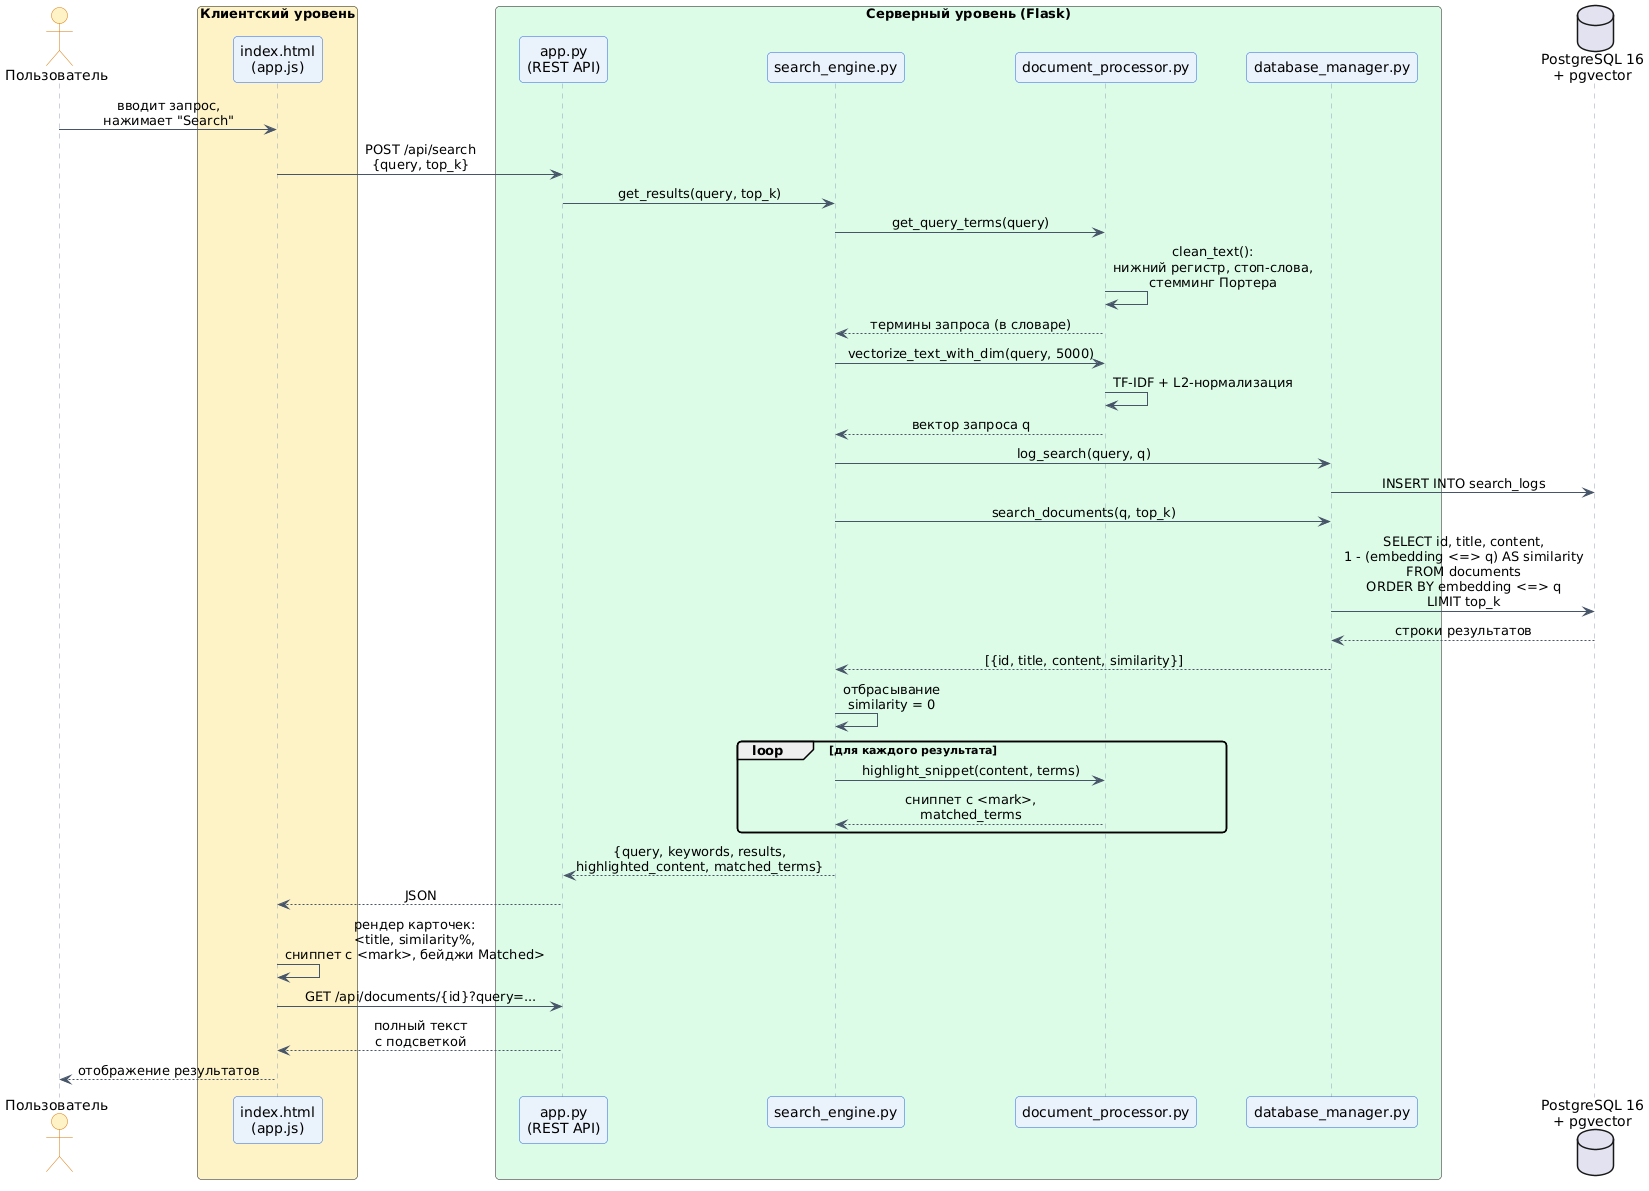
\includegraphics[width=1.0\textwidth]{png/sequence_search.png}
	\caption{Диаграмма последовательности обработки поискового запроса.}
	\label{fig:architecture}
\end{figure}

Серверная часть разбита на модули по принципу разделения ответственности:

\begin{itemize}
	\item \texttt{app.py} "--- точка входа; регистрирует REST-эндпоинты (\texttt{/api/search}, \texttt{/api/upload}, \texttt{/api/upload-file}, \texttt{/api/documents}, \texttt{/api/documents/<id>/download}, \texttt{/api/metrics}, \texttt{/api/stats}, \texttt{/api/help}, \texttt{/api/init-db}) и раздаёт статические страницы; при старте инициализирует bucket MinIO;
	\item \texttt{search\_engine.py} "--- оркестрация поиска: векторизация запроса, вызов векторного поиска в БД, формирование сниппетов с подсветкой релевантных терминов;
	\item \texttt{document\_processor.py} "--- предобработка текста, построение словаря, вычисление IDF, TF-IDF-векторизация, подсветка терминов;
	\item \texttt{document\_loader.py} "--- стратегия загрузки файлов: извлечение текста из различных форматов (\texttt{.txt}, \texttt{.md}, \texttt{.pdf}, \texttt{.docx}, \texttt{.html}, \texttt{.rtf}, \texttt{.csv}, \texttt{.log});
	\item \texttt{database\_manager.py} "--- все операции с PostgreSQL: CRUD документов (включая колонку \texttt{s3\_key} для хранения ключа в MinIO), векторный поиск, логирование запросов, сохранение/загрузка словаря и IDF;
	\item \texttt{s3\_client.py} "--- S3-клиент для MinIO: загрузка файлов (\texttt{upload\_file}), скачивание (\texttt{download\_file}), генерация presigned URL, проверка существования объектов, управление bucket;
	\item \texttt{evaluator.py} "--- вычисление метрик качества (точность, полнота, F-меры) и построение графиков;
	\item \texttt{watch\_handler.py} "--- серверная обработка событий файлового наблюдателя: извлечение текста, сохранение оригинального файла в MinIO, пересчёт словаря/IDF, генерация саммари, векторизация и upsert/delete документа;
	\item \texttt{migrate.py} "--- собственный раннер SQL-миграций, отслеживающий применённые миграции в таблице \texttt{schema\_migrations}.
\end{itemize}

Клиентский уровень реализован пятью статическими страницами: поиск (\texttt{index.html}),
загрузка документов (\texttt{upload.html}), просмотр документов (\texttt{documents.html}),
оценка качества (\texttt{metrics.html}) и справка (\texttt{help.html}). Взаимодействие
с сервером осуществляется через \texttt{fetch} по REST API с JSON-телом.

\subsection{Файловый наблюдатель (File Watcher)}

Для автоматической репликации изменений файловой системы на сервер реализован
отдельный CLI-клиент (\texttt{file\_watcher/watch\_client.py}), работающий на базе
библиотеки \texttt{watchdog}. Клиент выполняется на стороне пользователя (вне Docker-контейнера)
и взаимодействует с сервером через HTTP POST-запросы к эндпоинту \texttt{/api/watch-event}.

Архитектура клиента включает три основных компонента:

\begin{itemize}
	\item \textbf{WatchEventHandler} "--- обработчик событий watchdog (\texttt{on\_created}, \texttt{on\_modified}, \texttt{on\_deleted}, \texttt{on\_moved}); фильтрует файлы по расширению, выполняет debounce-задержку и отправляет HTTP POST на сервер;
	\item \textbf{WatchState} "--- персистентное состояние в файле \texttt{.watch\_state.json} (путь \texttt{<dir>/.watch\_state.json}); хранит \texttt{\{filepath: \{mtime, size\}\}} для каждого индексированного файла; при запуске клиент сравнивает текущее состояние файловой системы с сохранённым и отправляет только разницу (новые, изменённые, удалённые файлы);
	\item \textbf{CLI (argparse)} "--- интерфейс командной строки с параметрами: директория, адрес сервера, client-id, рекурсивный режим, расширения файлов, debounce, путь к state-файлу.
\end{itemize}

Потоки данных клиента:

\begin{enumerate}
	\item \textbf{При запуске:} загрузка \texttt{.watch\_state.json}, сканирование директории (\texttt{os.walk}), сравнение с сохранённым состоянием, отправка diff'а (new/changed/deleted) серверу, обновление state-файла;
	\item \textbf{При работе:} watchdog Observer отслеживает события в реальном времени; при каждом событии (\texttt{on\_created}/\texttt{on\_modified}/\texttt{on\_deleted}) клиент отправляет POST-запрос на сервер и обновляет \texttt{.watch\_state.json}.
\end{enumerate}

На сервере обработка событий выполняется модулем \texttt{watch\_handler.py}, который
вызывается из REST API (\texttt{/api/watch-event}). Для событий \texttt{created} и
\texttt{modified}: извлекается текст (через \texttt{document\_loader.py}), пересчитываются
словарь и IDF по всему корпусу, генерируется саммари, вычисляется TF-IDF-вектор и
выполняется upsert документа в БД. Для события \texttt{deleted}: документ удаляется
по \texttt{file\_path}, после чего пересчитываются словарь и IDF.

Последовательность взаимодействия компонентов при работе файлового наблюдателя
приведена на рисунке~\ref{fig:watch_seq}.

\begin{figure}[H]
	\centering
	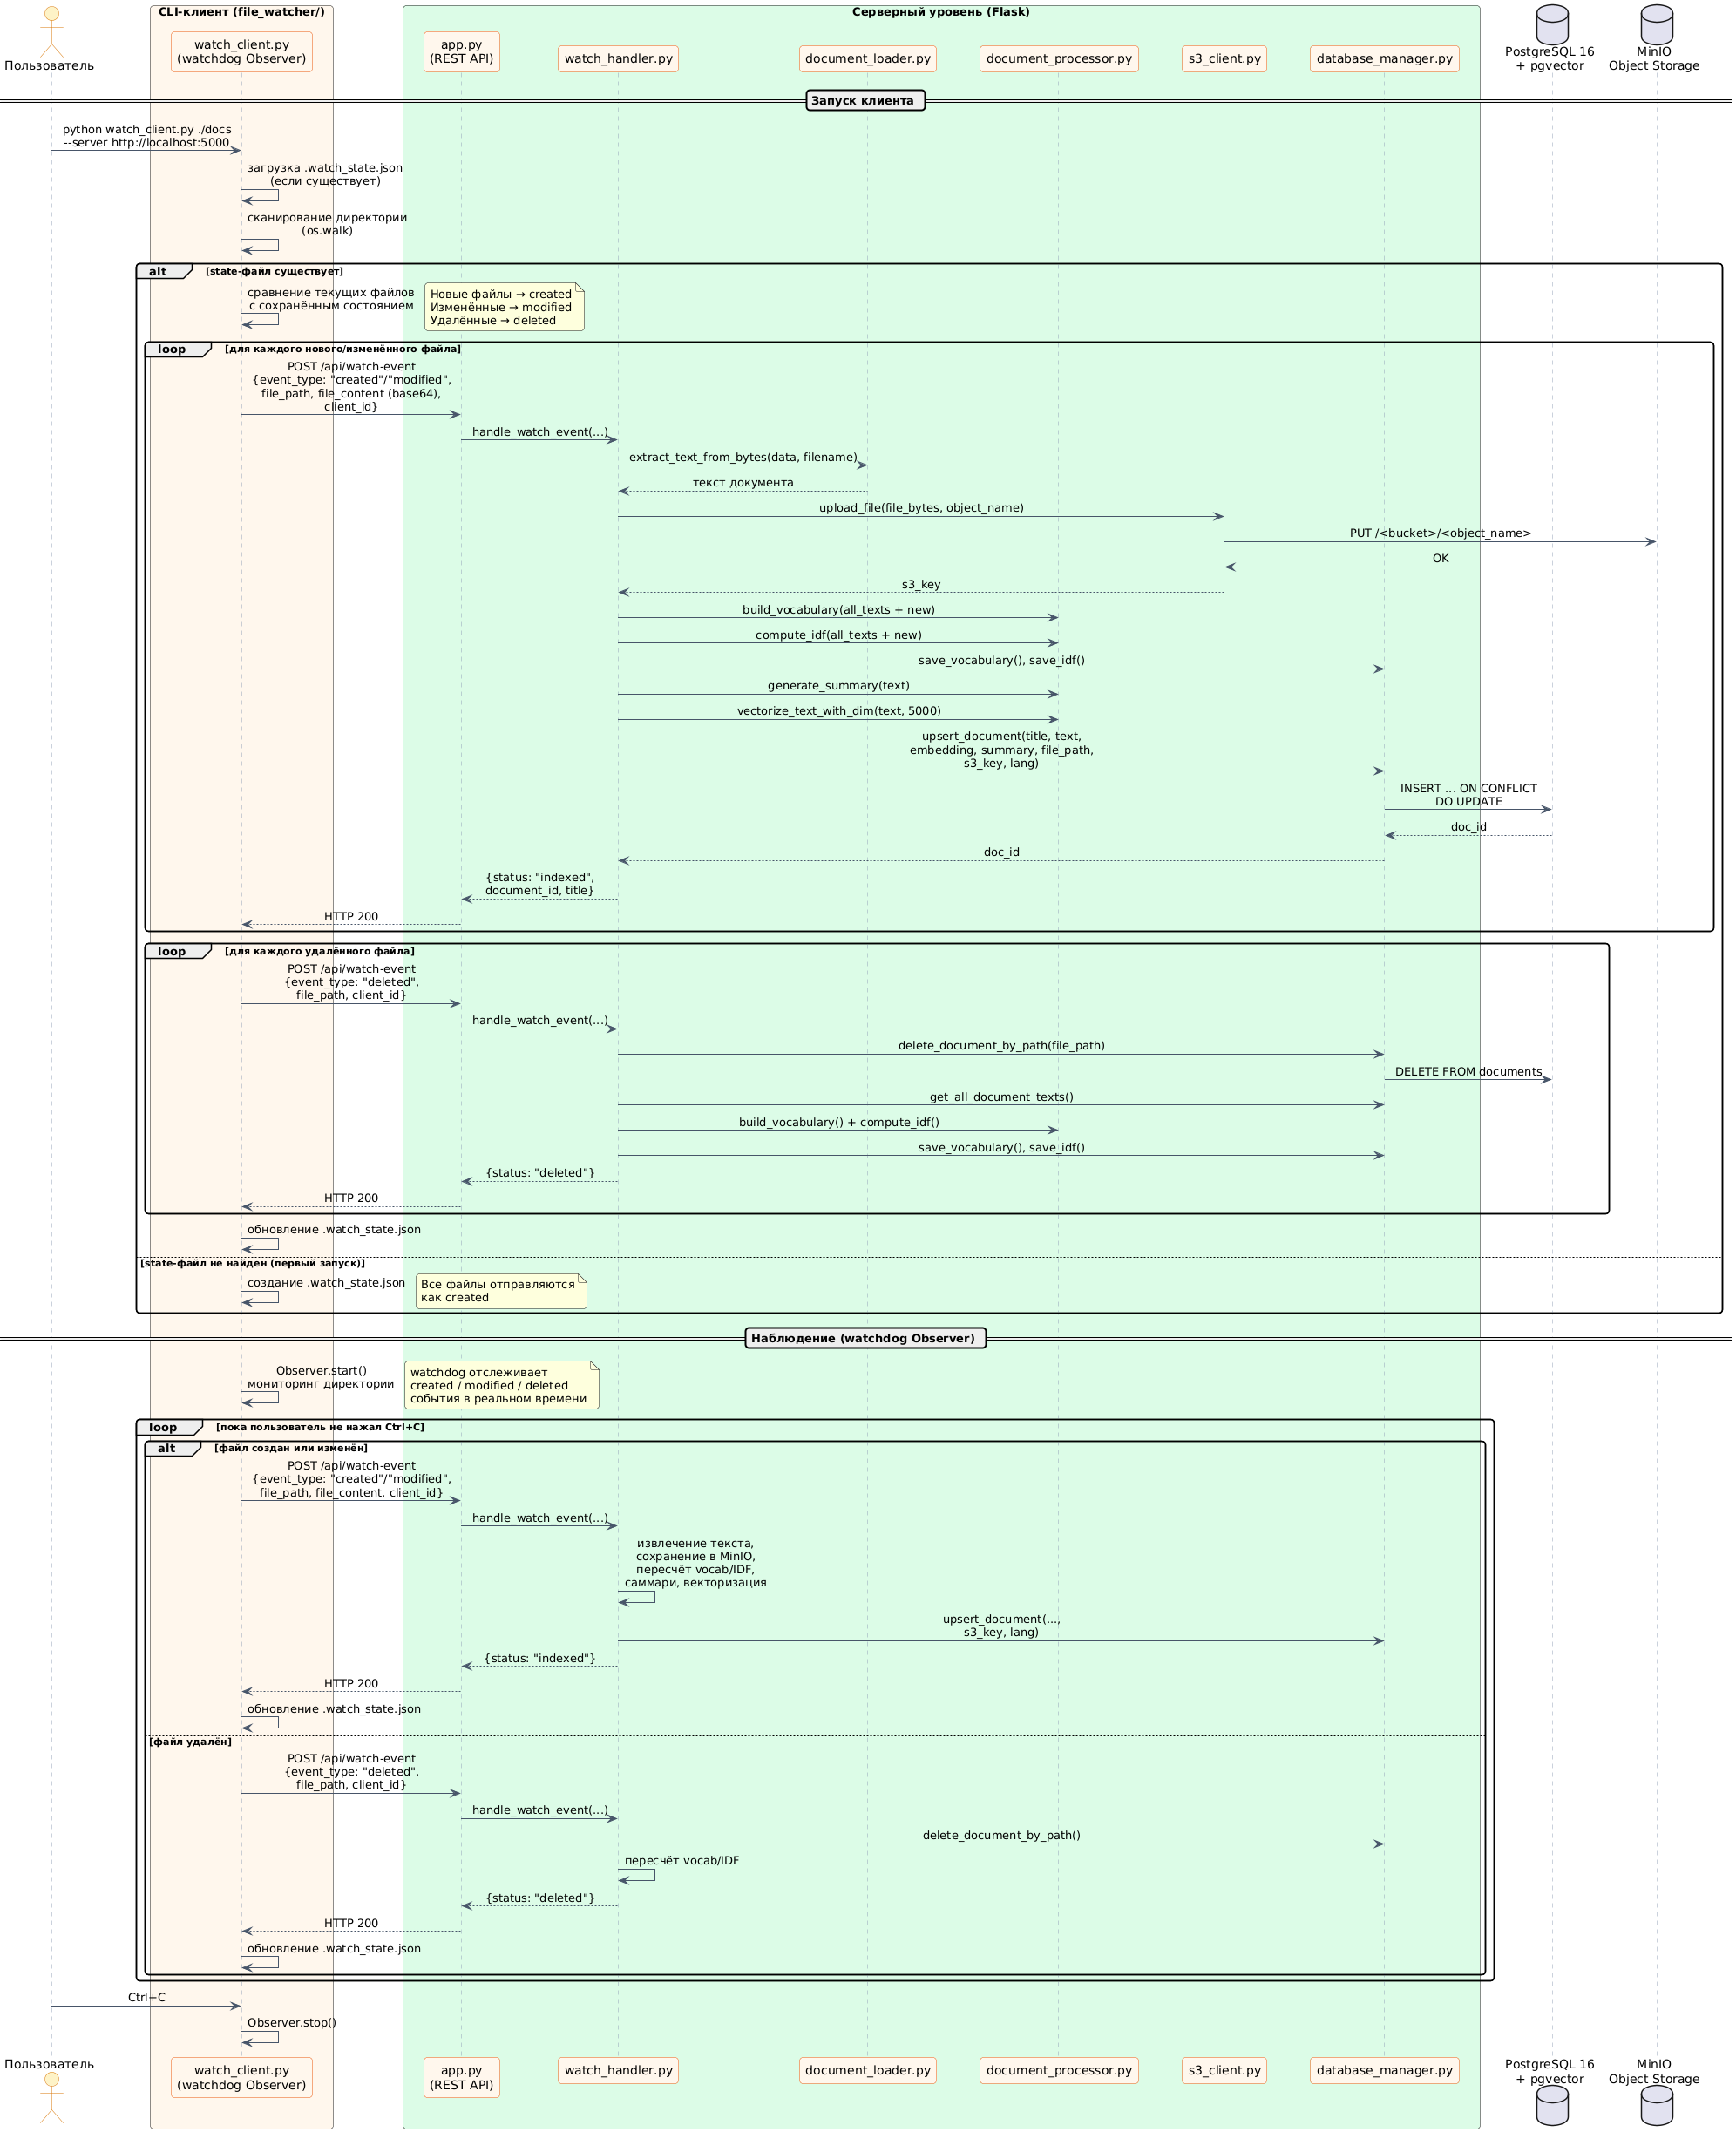
\includegraphics[width=1.0\textwidth]{png/sequence_watch.png}
	\caption{Диаграмма последовательности работы файлового наблюдателя.}
	\label{fig:watch_seq}
\end{figure}

\subsection{Хранение и скачивание документов (MinIO S3)}

Для хранения оригинальных файлов документов используется MinIO Object Storage "--- 
S3-совместимое хранилище объектов. При загрузке файла через \texttt{/api/upload-file}
или при обработке событий файлового наблюдателя оригинальный файл сохраняется в MinIO
(bucket \texttt{documents}), а в таблицу \texttt{documents} записывается ключ объекта
(\texttt{s3\_key}) в формате \texttt{<uuid>.<ext>}.

Скачивание документов реализовано через эндпоинт \texttt{/api/documents/<id>/download}.
При наличии \texttt{s3\_key} файл скачивается из MinIO через \texttt{s3\_client.py}
и отдаётся пользователю с заголовком \texttt{Content-Disposition: attachment}, что
обеспечивает скачивание файла вместо отображения в браузере. Для старых документов
без \texttt{s3\_key} (загруженных через текстовый ввод) генерируется \texttt{.txt}-файл
на лету из сохранённого текста.

Архитектура взаимодействия при скачивании документа представлена на рисунке~\ref{fig:download_seq}.

\begin{figure}[H]
	\centering
	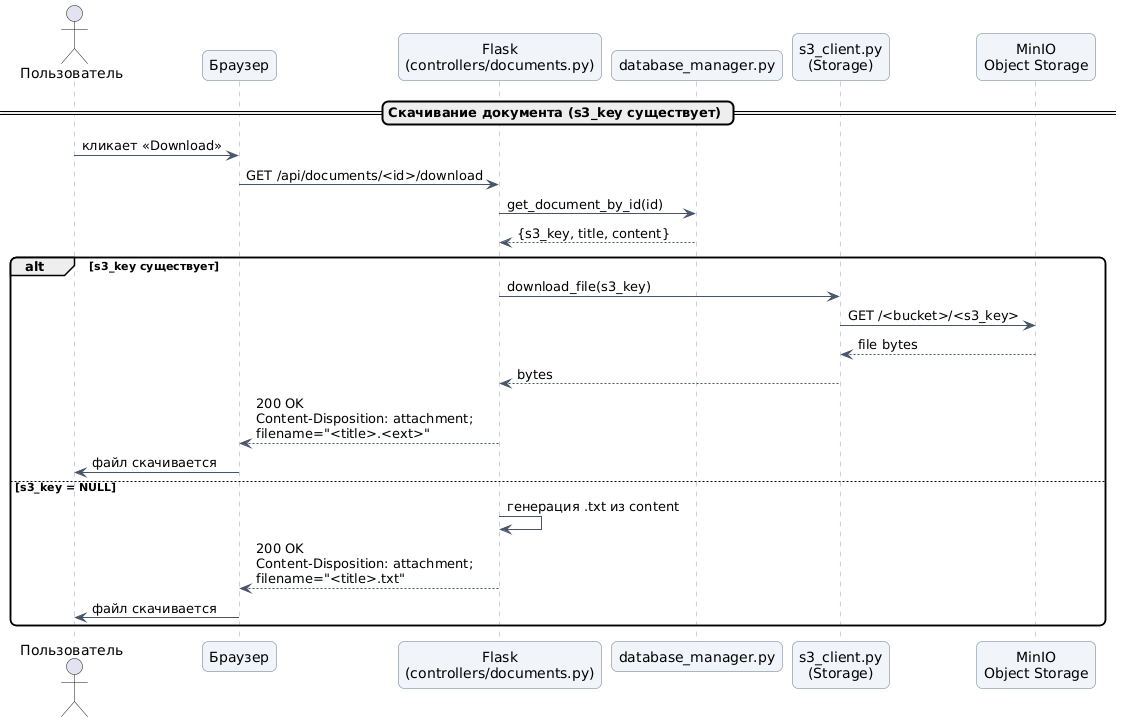
\includegraphics[width=1.0\textwidth]{png/sequence_download.png}
	\caption{Диаграмма последовательности скачивания документа из MinIO.}
	\label{fig:download_seq}
\end{figure}

Последовательность загрузки файла в MinIO при загрузке через веб-интерфейс
представлена на рисунке~\ref{fig:upload_file_seq}.

\begin{figure}[H]
	\centering
	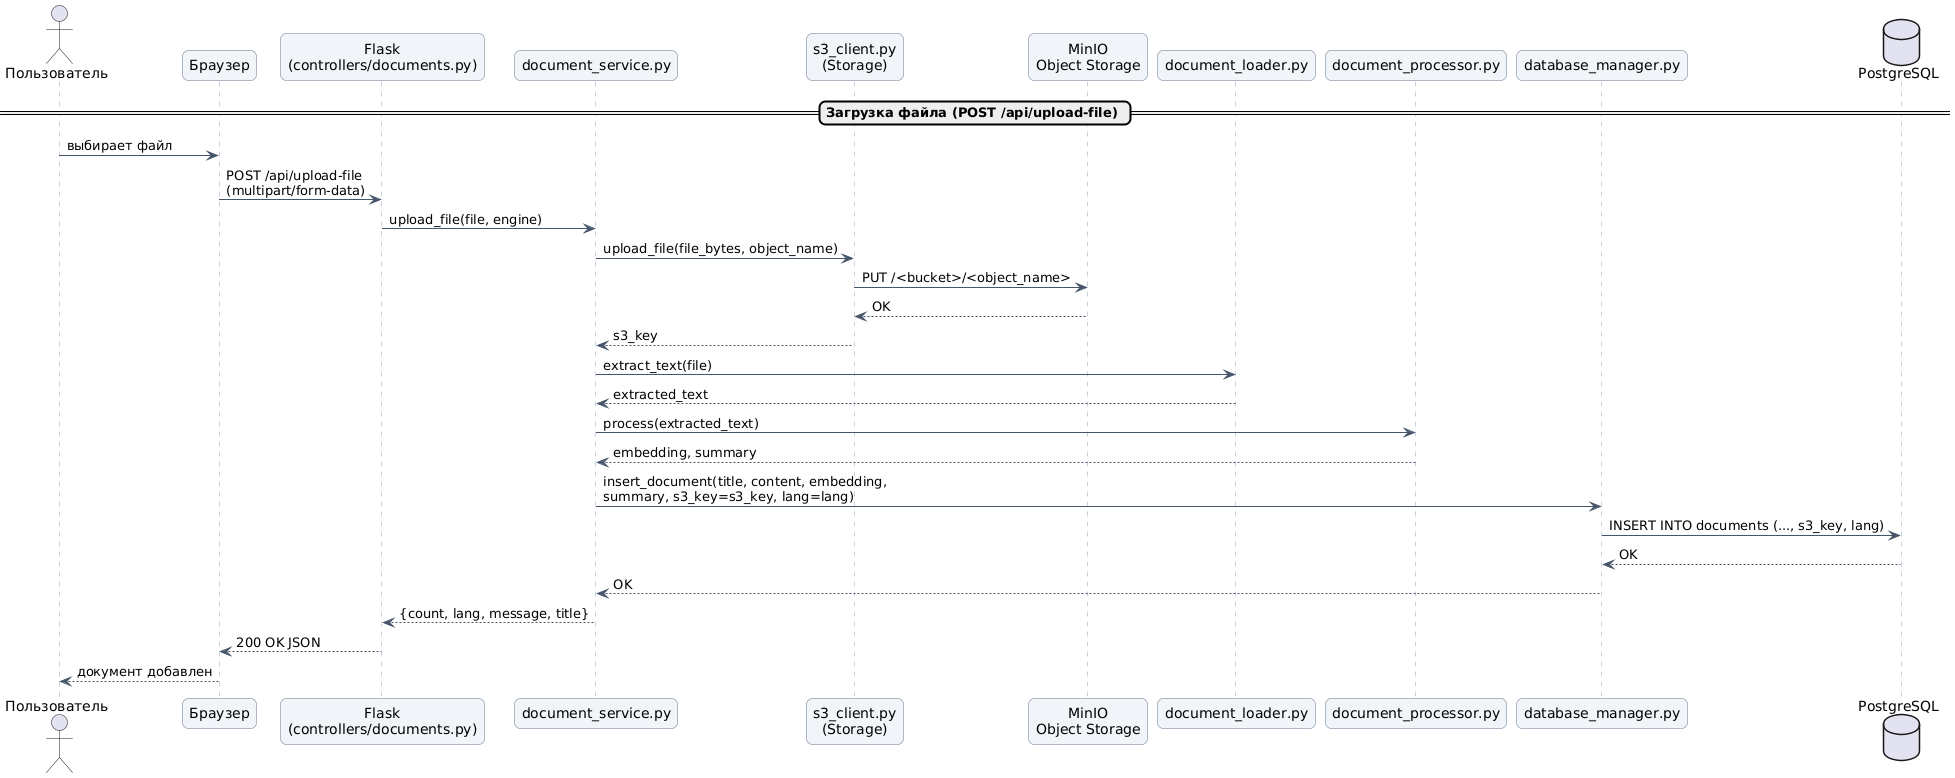
\includegraphics[width=1.0\textwidth]{png/sequence_upload_file.png}
	\caption{Диаграмма последовательности загрузки файла с сохранением в MinIO.}
	\label{fig:upload_file_seq}
\end{figure}

Развёртывание выполняется в Docker Compose: сервис \texttt{db} (образ \texttt{pgvector/pgvector:pg16}),
сервис \texttt{app} (образ на основе \texttt{python:3.11-slim}) и сервис \texttt{minio}
(образ \texttt{quay.io/minio/minio}). При старте контейнера \texttt{app} ожидается
готовность базы данных, применяются миграции, создаётся bucket \texttt{documents} в MinIO,
запускается Flask, а затем автоматически инициализируется корпус документов (если база пуста).
Приложение доступно по \texttt{http://<host>:5000}, MinIO Console "--- по \texttt{http://<host>:9001},
что позволяет использовать систему в локальной вычислительной сети.

\subsection{Структура базы данных системы}

База данных содержит семь таблиц, перечисленных в таблице~\ref{tab:db_tables}.

\begin{table}[H]
	\centering
	\begin{tabular}{|p{3.2cm}|p{8.8cm}|}
		\hline
		\textbf{Таблица} & \textbf{Назначение} \\
		\hline
		\texttt{documents} & Индексированные документы: идентификатор, заголовок, полный текст, дата добавления, TF-IDF-вектор размерности 5000, саммари, путь к файлу, код языка (\texttt{lang}: \texttt{en}/\texttt{fr}), ключ объекта в MinIO (\texttt{s3\_key}) \\
		\hline
		\texttt{search\_logs} & Логи поисковых запросов: текст запроса, вектор запроса, время \\
		\hline
		\texttt{vocabulary} & Словарь терминов: слово и его индекс в векторе \\
		\hline
		\texttt{idf\_values} & Инверсные документные частоты терминов словаря \\
		\hline
		\texttt{schema\_migrations} & Служебная таблица учёта применённых миграций \\
		\hline
		\texttt{watch\_clients} & Зарегистрированные клиенты-наблюдатели: ID, наблюдаемая директория, время регистрации \\
		\hline
		\texttt{watch\_events} & Логи событий файлового наблюдателя: тип события, путь к файлу, время \\
		\hline
	\end{tabular}
	\caption{Таблицы базы данных и их назначение.}
	\label{tab:db_tables}
\end{table}

Словарь и IDF-значения хранятся в базе данных для персистентности между перезапусками
приложения, однако при выполнении поиска используются их in-memory копии (глобальные
структуры \texttt{VOCAB} и \texttt{IDF}), что исключает обращения к БД при каждом
векторном поиске.

\subsection{Основные алгоритмы реализации компонентов}

\textbf{Предобработка текста.} Исходный текст приводится к нижнему регистру, из него
удаляются цифры, пунктуация и спецсимволы; для французского режима сохраняются
диакритические символы (\texttt{àâäéèêëîïôöùûüç"{o}e}). Затем токены
фильтруются по списку стоп-слов (соответствующий набор для каждого языка
из NLTK) и стеммируются алгоритмом Портера (только для английского;
французский текст не стемминуется, чтобы сохранить окончания). Параметр
\texttt{lang} устанавливается автоматически при загрузке документа
(классификатор записывает результат в колонку \texttt{lang} таблицы
\texttt{documents}) и при поиске определяется для запроса тем же
классификатором. Результат "--- список основ терминов, из которых
строятся векторы.

\textbf{Построение словаря и вычисление IDF.} Словарь формируется как упорядоченное
множество уникальных терминов корпуса; мощность словаря определяет размерность
векторного пространства $D$. Инверсная документная частота вычисляется по формуле:

\begin{equation}
	B_{i} = \log\left(\frac{N}{P_{i} + 1}\right) + 1,
	\label{eq:idf}
\end{equation}

где $N$ "--- число документов в коллекции; $P_{i}$ "--- число документов, содержащих
термин $i$. Добавление единицы в знаменатель и к результату устраняет нулевые значения
для терминов, встречающихся во всех документах, сохраняя свойство убывания значимости
частых терминов.

\textbf{TF-IDF-векторизация.} Вес термина $i$ в документе $j$ вычисляется по формуле:

\begin{equation}
	A^{j}_{i} = Q^{j}_{i} \times B_{i},
	\label{eq:weight}
\end{equation}

где $Q^{j}_{i} = 1 + \log\left(\text{tf}^{j}_{i}\right)$ "--- сглаженная частота термина
в документе (логарифмическая нормализация снижает влияние часто повторяющихся слов).
Полученный вектор нормируется евклидовой нормой:

\begin{equation}
	\vec{v} = \frac{\vec{w}}{\lVert \vec{w} \rVert}.
	\label{eq:norm}
\end{equation}

Ключевой фрагмент векторизации приведён в листинге~\ref{lst:vectorize}.

\begin{lstlisting}[caption={Функция TF-IDF-векторизации текста.},label={lst:vectorize}]
def vectorize_text_with_dim(text: str, dim: int, lang: str = 'en') -> List[float]:
    tokens = clean_text(text, lang)
    tf = Counter(tokens)
    vector = [0.0] * dim
    for token, count in tf.items():
        if token in VOCAB:
            idx = VOCAB[token]
            if idx < dim:
                tf_val = 1 + math.log(count) if count > 0 else 0
                idf_val = IDF.get(token, math.log(10) + 1)
                vector[idx] = tf_val * idf_val
    norm = math.sqrt(sum(v * v for v in vector))
    if norm > 0:
        vector = [v / norm for v in vector]
    return vector
\end{lstlisting}

\textbf{Модель поиска.} Запрос пользователя обрабатывается той же функцией
векторизации, что и документы, после чего релевантность документа $d$ запросу $q$
оценивается косинусной близостью соответствующих векторов:

\begin{equation}
	\operatorname{sim}(d, q) = \frac{(\vec{D}, \vec{Q})}{\lVert \vec{D} \rVert \cdot \lVert \vec{Q} \rVert}.
	\label{eq:cosine}
\end{equation}

Поскольку документные векторы нормированы, косинусная близость равна скалярному
произведению. В СУБД это реализовано оператором pgvector \texttt{<=>} (косинусное
расстояние), а итоговая оценка близости вычисляется как разность единицы и косинусного
расстояния (листинг~\ref{lst:search}): $\operatorname{sim}(d,q) = 1 - d_{\cos}(\vec{D}, \vec{Q})$.

\begin{lstlisting}[caption={Векторный поиск в PostgreSQL (pgvector).},label={lst:search}]
SELECT id, title, content,
       1 - (embedding <=> %s::vector) AS similarity
FROM documents
ORDER BY embedding <=> %s::vector
LIMIT %s
\end{lstlisting}

Результаты с нулевой близостью отбрасываются: они не несут информации для
пользователя и засоряют выдачу.

\textbf{Подсветка релевантных терминов.} Для каждого результата строится сниппет:
находится первое вхождение термина запроса (после стемминга), вокруг него выделяется
окно фиксированной длины с многоточиями по краям, а все совпавшие термины оборачиваются
в HTML-тег \texttt{<mark>}. Если ни один термин запроса не встречается в документе,
подсвечиваются ключевые термины самого документа (по весу TF-IDF). Подсветка также
применяется при просмотре полного текста документа по клику.

\textbf{Загрузка документов.} Модуль \texttt{document\_loader.py} реализует стратегию
извлечения текста по расширению файла: текстовые форматы декодируются с перебором
кодировок (UTF-8, CP1251, Latin-1), HTML очищается от тегов и скриптов, RTF "--- от
управляющих слов, PDF и DOCX обрабатываются библиотеками pypdf и python-docx.
Поддерживаемые форматы перечислены в таблице~\ref{tab:formats}.

\begin{table}[H]
	\centering
	\begin{tabular}{|p{4.5cm}|p{7.5cm}|}
		\hline
		\textbf{Расширение} & \textbf{Механизм извлечения текста} \\
		\hline
		\texttt{.txt}, \texttt{.md}, \texttt{.csv}, \texttt{.log} & декодирование с перебором кодировок \\
		\hline
		\texttt{.pdf} & библиотека pypdf (постраничное извлечение) \\
		\hline
		\texttt{.docx} & библиотека python-docx (абзацы и таблицы) \\
		\hline
		\texttt{.html}, \texttt{.htm} & удаление тегов и script/style-блоков \\
		\hline
		\texttt{.rtf} & удаление управляющих слов RTF \\
		\hline
	\end{tabular}
	\caption{Поддерживаемые форматы загружаемых документов.}
	\label{tab:formats}
\end{table}

При загрузке каждого нового документа определяется его язык трёхметодным
классификатором (результат записывается в колонку \texttt{lang} таблицы
\texttt{documents}); далее словарь и IDF пересчитываются по всему корпусу
и сохраняются в базу данных, после чего документ индексируется (его TF-IDF-вектор
вставляется в таблицу \texttt{documents}). Последовательность взаимодействия компонентов
при индексировании документа приведена на рисунке~\ref{fig:indexing}.

\begin{figure}[H]
	\centering
	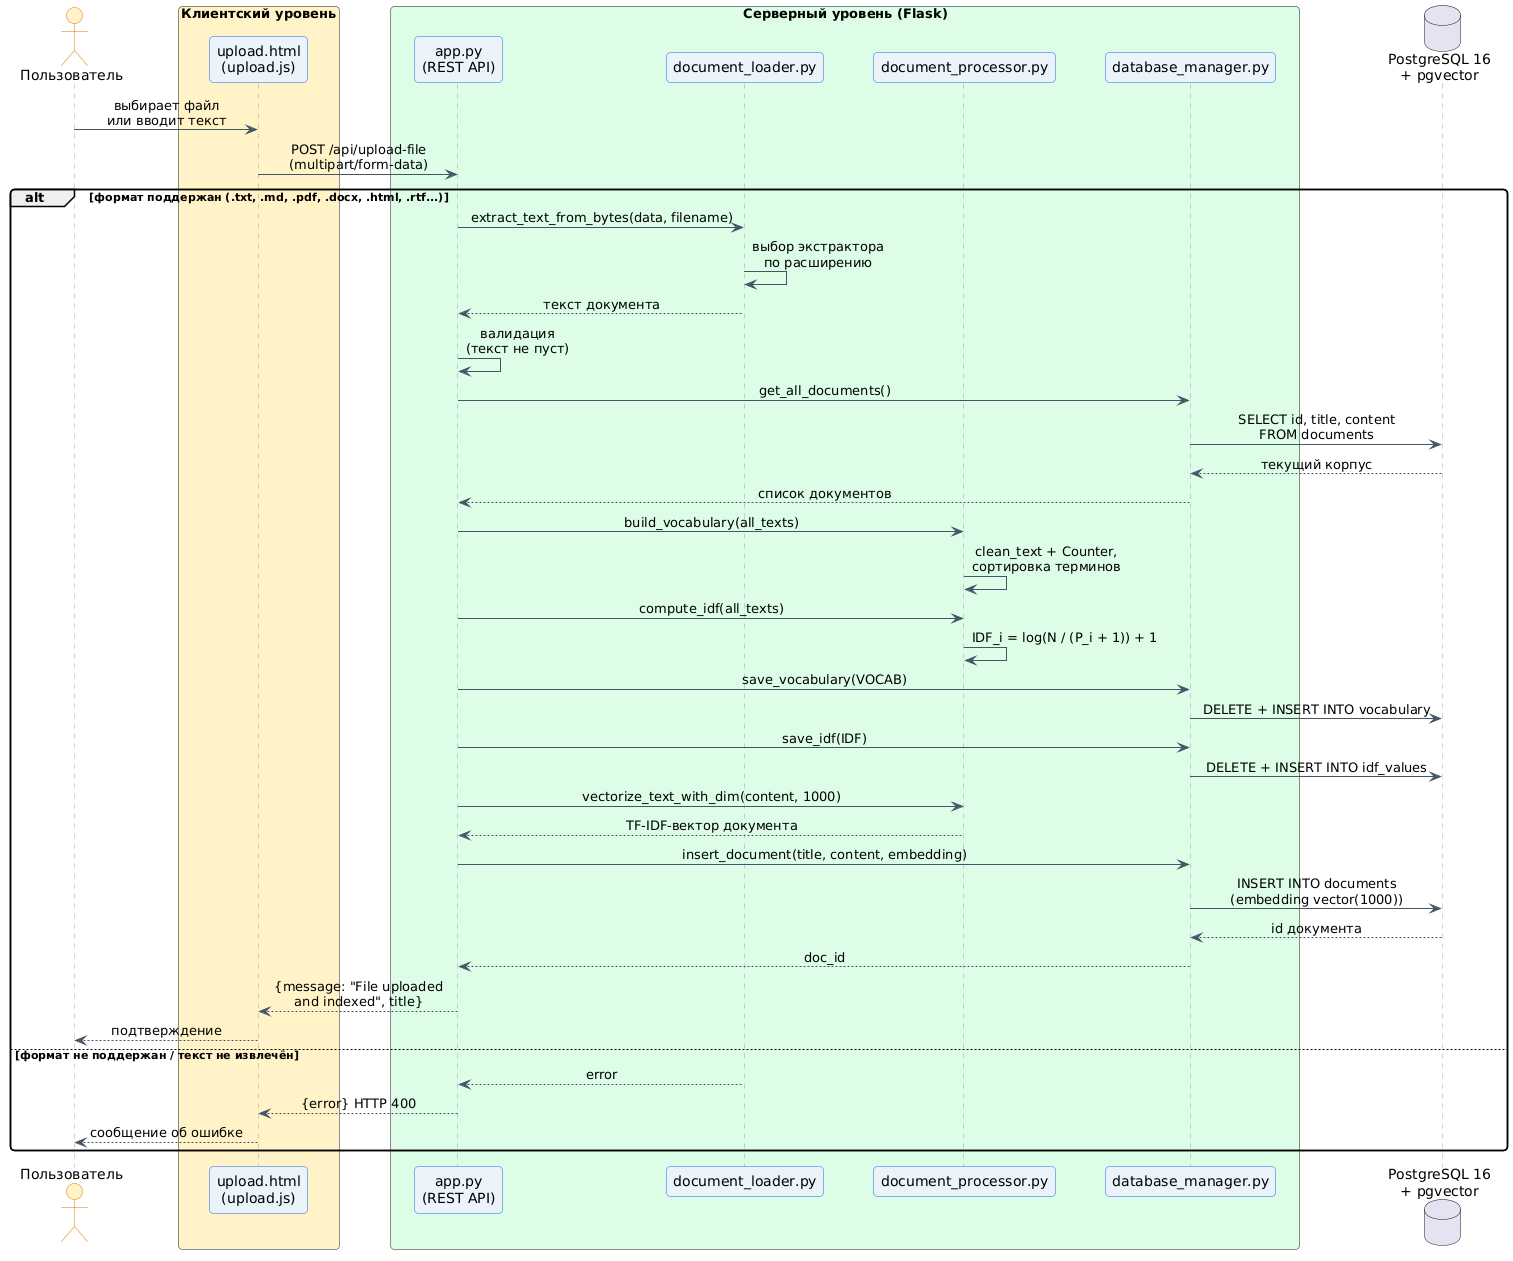
\includegraphics[width=1.0\textwidth]{png/sequense_indexing.png}
	\caption{Диаграмма последовательности индексирования документа.}
	\label{fig:indexing}
\end{figure}

\textbf{Оценка качества поиска.} Для оценки качества используются метрики точности,
полноты и F-меры, вычисляемые по множествам выданных и релевантных документов:

\begin{equation}
	P = \frac{|R \cap Rel|}{|R|}, \qquad
	R = \frac{|R \cap Rel|}{|Rel|},
	\label{eq:pr}
\end{equation}

\begin{equation}
	F_{\beta} = \frac{(1 + \beta^{2}) \cdot P \cdot R}{\beta^{2} \cdot P + R}.
	\label{eq:fbeta}
\end{equation}

Параметр $\beta$ позволяет сместить акцент: $\beta = 0{,}5$ "--- важнее точность,
$\beta = 1$ "--- сбалансированная F1-мера, $\beta = 2$ "--- важнее полнота.
Оценка выполняется автоматически: для каждого тестового запроса выполняется реальный
поиск (извлекаются \texttt{retrieved\_ids}), которые сравниваются с эталонными
релевантными документами, заданными пользователем на странице \texttt{metrics.html}.
Последовательность взаимодействия компонентов при оценке качества приведена
на рисунке~\ref{fig:metrics_seq}.

\begin{figure}[H]
	\centering
	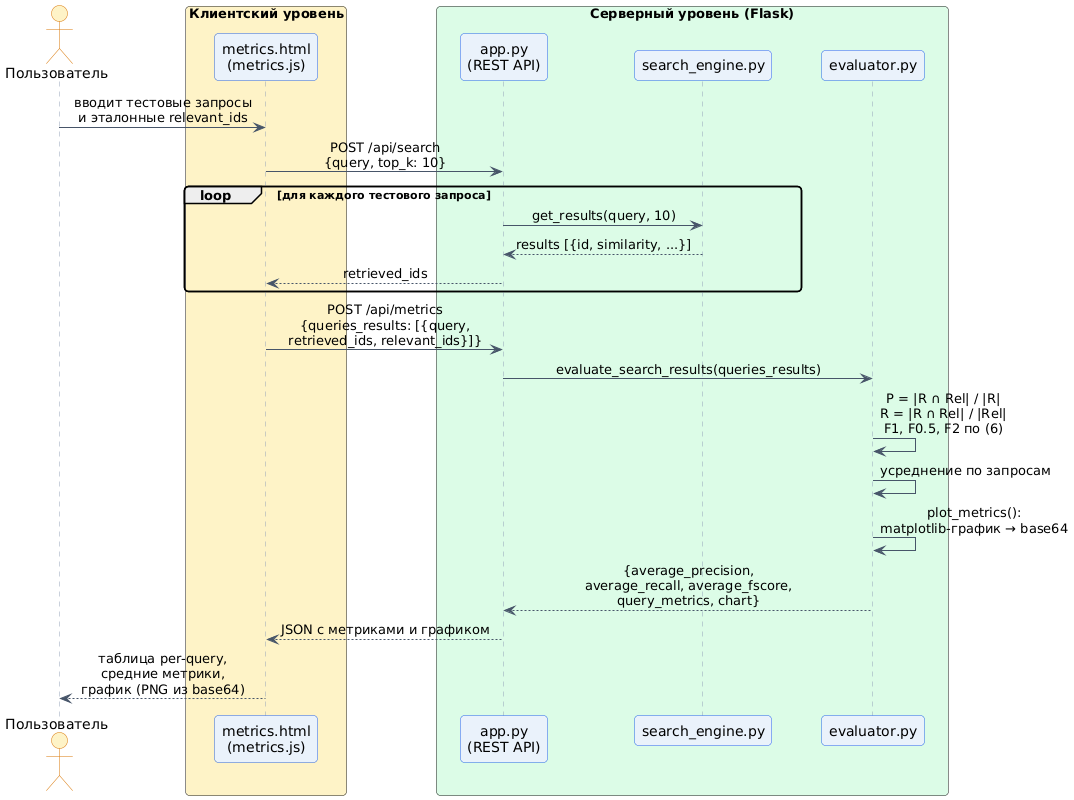
\includegraphics[width=1.0\textwidth]{png/sequence_metrics.png}
	\caption{Диаграмма последовательности оценки качества поиска.}
	\label{fig:metrics_seq}
\end{figure}

\subsection{Информация о тестовой коллекции документов}

Тестовая коллекция состоит из 12 текстовых документов на английском языке объёмом
по 300 "--- 600 слов каждый, посвящённых тематике музыки. Перечень документов приведён
в таблице~\ref{tab:collection}.

\begin{table}[H]
	\centering
	\begin{tabular}{|c|p{4.8cm}|p{6.8cm}|}
		\hline
		\textbf{ID} & \textbf{Документ} & \textbf{Тематика} \\
		\hline
		1 & blues\_music & блюз: происхождение, исполнители, влияние \\
		\hline
		2 & classical\_music & классическая музыка: эпохи, композиторы \\
		\hline
		3 & electronic\_music & электронная музыка: синтезаторы, жанры \\
		\hline
		4 & jazz\_music & джаз: история, инструменты, музыканты \\
		\hline
		5 & music\_concerts & концерты: организация, живое исполнение \\
		\hline
		6 & music\_education & музыкальное образование и обучение \\
		\hline
		7 & music\_industry & музыкальная индустрия и бизнес \\
		\hline
		8 & music\_instruments & музыкальные инструменты и их классификация \\
		\hline
		9 & music\_production & музыкальное производство и запись \\
		\hline
		10 & music\_theory & теория музыки: ритм, мелодия, гармония \\
		\hline
		11 & pop\_music & популярная музыка и её особенности \\
		\hline
		12 & rock\_music & рок-музыка: жанры, инструменты, история \\
		\hline
	\end{tabular}
	\caption{Тестовая коллекция документов.}
	\label{tab:collection}
\end{table}

Документы загружаются в систему автоматически при первой инициализации базы данных
(\texttt{/api/init-db}) и хранятся в каталоге \texttt{backend/documents/} в формате
\texttt{.txt}.

\subsection{Результаты тестирования системы}

Тестирование проводилось вручную по следующим сценариям:

\begin{enumerate}
	\item инициализация базы данных: миграции применяются в правильном порядке, корпус из 12 документов загружается автоматически при пустой базе и не дублируется при повторных стартах;
	\item поиск по запросам различной длины: одиночный термин, многокомпонентный запрос, запрос с отсутствующими в корпусе словами; проверялись релевантность выдачи, корректность процента близости и отбрасывание нулевых результатов;
	\item подсветка релевантных терминов: в сниппетах и в полном тексте документа помечаются термины запроса; для документов без совпадений применяется фолбэк по ключевым терминам документа;
	\item загрузка документов: ручной ввод текста, загрузка \texttt{.txt}, \texttt{.pdf}, \texttt{.docx}, \texttt{.html}; проверялось извлечение текста и индексация; неподдерживаемый формат (например, \texttt{.png}) отклоняется с понятным сообщением;
	\item просмотр и удаление документов: список с идентификаторами, открытие полного текста, удаление;
	\item скачивание документов: для документов с \texttt{s3\_key} файл скачивается из MinIO с заголовком \texttt{Content-Disposition: attachment}; для документов без \texttt{s3\_key} генерируется \texttt{.txt}-файл на лету;
	\item оценка качества: для набора тестовых запросов рассчитываются точность, полнота и F-меры, строится график;
	\item файловый наблюдатель: запуск клиента с наблюдаемой директорией; проверяется автоматическая индексация новых файлов, обновление изменённых, удаление удалённых; проверяется корректность state-файла при перезапуске;
	\item отказоустойчивость: недоступность базы данных, пустой запрос, пустой файл, файл без извлекаемого текста.
\end{enumerate}

В ходе тестирования были выявлены и устранены следующие дефекты:

\begin{itemize}
	\item страница оценки метрик отправляла на сервер поле \texttt{relevantIds} вместо ожидаемого \texttt{relevant\_ids} и не передавала \texttt{retrieved\_ids}, из-за чего сервер завершался с ошибкой \texttt{KeyError}; исправлено: фронтенд выполняет реальный поиск и передаёт оба списка, на сервере добавлен фолбэк "--- при отсутствии \texttt{retrieved\_ids} поиск выполняется автоматически;
	\item сниппеты результатов обрезались до 500 символов на уровне SQL-запроса, что не позволяло строить осмысленную подсветку; полный текст теперь возвращается целиком, а обрезка выполняется при формировании сниппета;
	\item при повторном старте контейнера корпус документов дублировался; добавлена проверка числа документов перед инициализацией.
\end{itemize}

Все сценарии после исправлений проходят успешно.

\subsection{Результаты оценки по метрикам}

Оценка выполнялась на тестовой коллекции из 12 документов. Для каждого из 11 тестовых
запросов задавалось эталонное множество релевантных документов (1 "--- 3 документа).
Система выполняла реальный поиск (топ-10), после чего вычислялись метрики. Результаты
приведены в таблице~\ref{tab:metrics}.

\begin{table}[H]
	\centering
	\begin{tabular}{|p{5.2cm}|c|c|c|c|c|}
		\hline
		\textbf{Запрос} & \textbf{P} & \textbf{R} & \textbf{F1} & \textbf{F0.5} & \textbf{F2} \\
		\hline
		jazz saxophone trumpet & 1,000 & 1,000 & 1,000 & 1,000 & 1,000 \\
		\hline
		blues & 0,667 & 1,000 & 0,800 & 0,714 & 0,909 \\
		\hline
		rock electric guitar & 0,500 & 1,000 & 0,667 & 0,556 & 0,833 \\
		\hline
		concerts live & 0,250 & 1,000 & 0,400 & 0,294 & 0,625 \\
		\hline
		classical music symphony & 0,200 & 1,000 & 0,333 & 0,238 & 0,556 \\
		\hline
		electronic music & 0,200 & 1,000 & 0,333 & 0,238 & 0,556 \\
		\hline
		pop music & 0,100 & 1,000 & 0,182 & 0,122 & 0,357 \\
		\hline
		music production recording & 0,100 & 1,000 & 0,182 & 0,122 & 0,357 \\
		\hline
		music theory harmony & 0,100 & 1,000 & 0,182 & 0,122 & 0,357 \\
		\hline
		music education & 0,100 & 1,000 & 0,182 & 0,122 & 0,357 \\
		\hline
		music industry & 0,100 & 1,000 & 0,182 & 0,122 & 0,357 \\
		\hline
		\textbf{Среднее} & \textbf{0,302} & \textbf{1,000} & \textbf{0,404} & \textbf{0,321} & \textbf{0,533} \\
		\hline
	\end{tabular}
	\caption{Метрики качества поиска по тестовым запросам.}
	\label{tab:metrics}
\end{table}

Аналитическая интерпретация. Полнота $R = 1{,}0$ для всех запросов: при небольшом
корпусе (12 документов) и выдаче из 10 результатов все эталонные релевантные документы
всегда попадают в топ-10, т.~е. система не теряет ни одного релевантного документа.
Точность $P$ убывает от 1,0 (запрос с редкими терминами \texttt{jazz saxophone trumpet})
до 0,1 (общие запросы \texttt{pop music}, \texttt{music theory harmony}), поскольку
документы корпуса тематически близки и делят значительную часть словаря "--- по общим
запросам в топ-10 попадает много нерелевантных документов с ненулевой близостью.
Средняя F1-мера составила 0,404: при идеальной полноте качество ограничивает именно
точность.

Графическое представление результатов приведено на рисунке~\ref{fig:metrics}.

\begin{figure}[H]
	\centering
	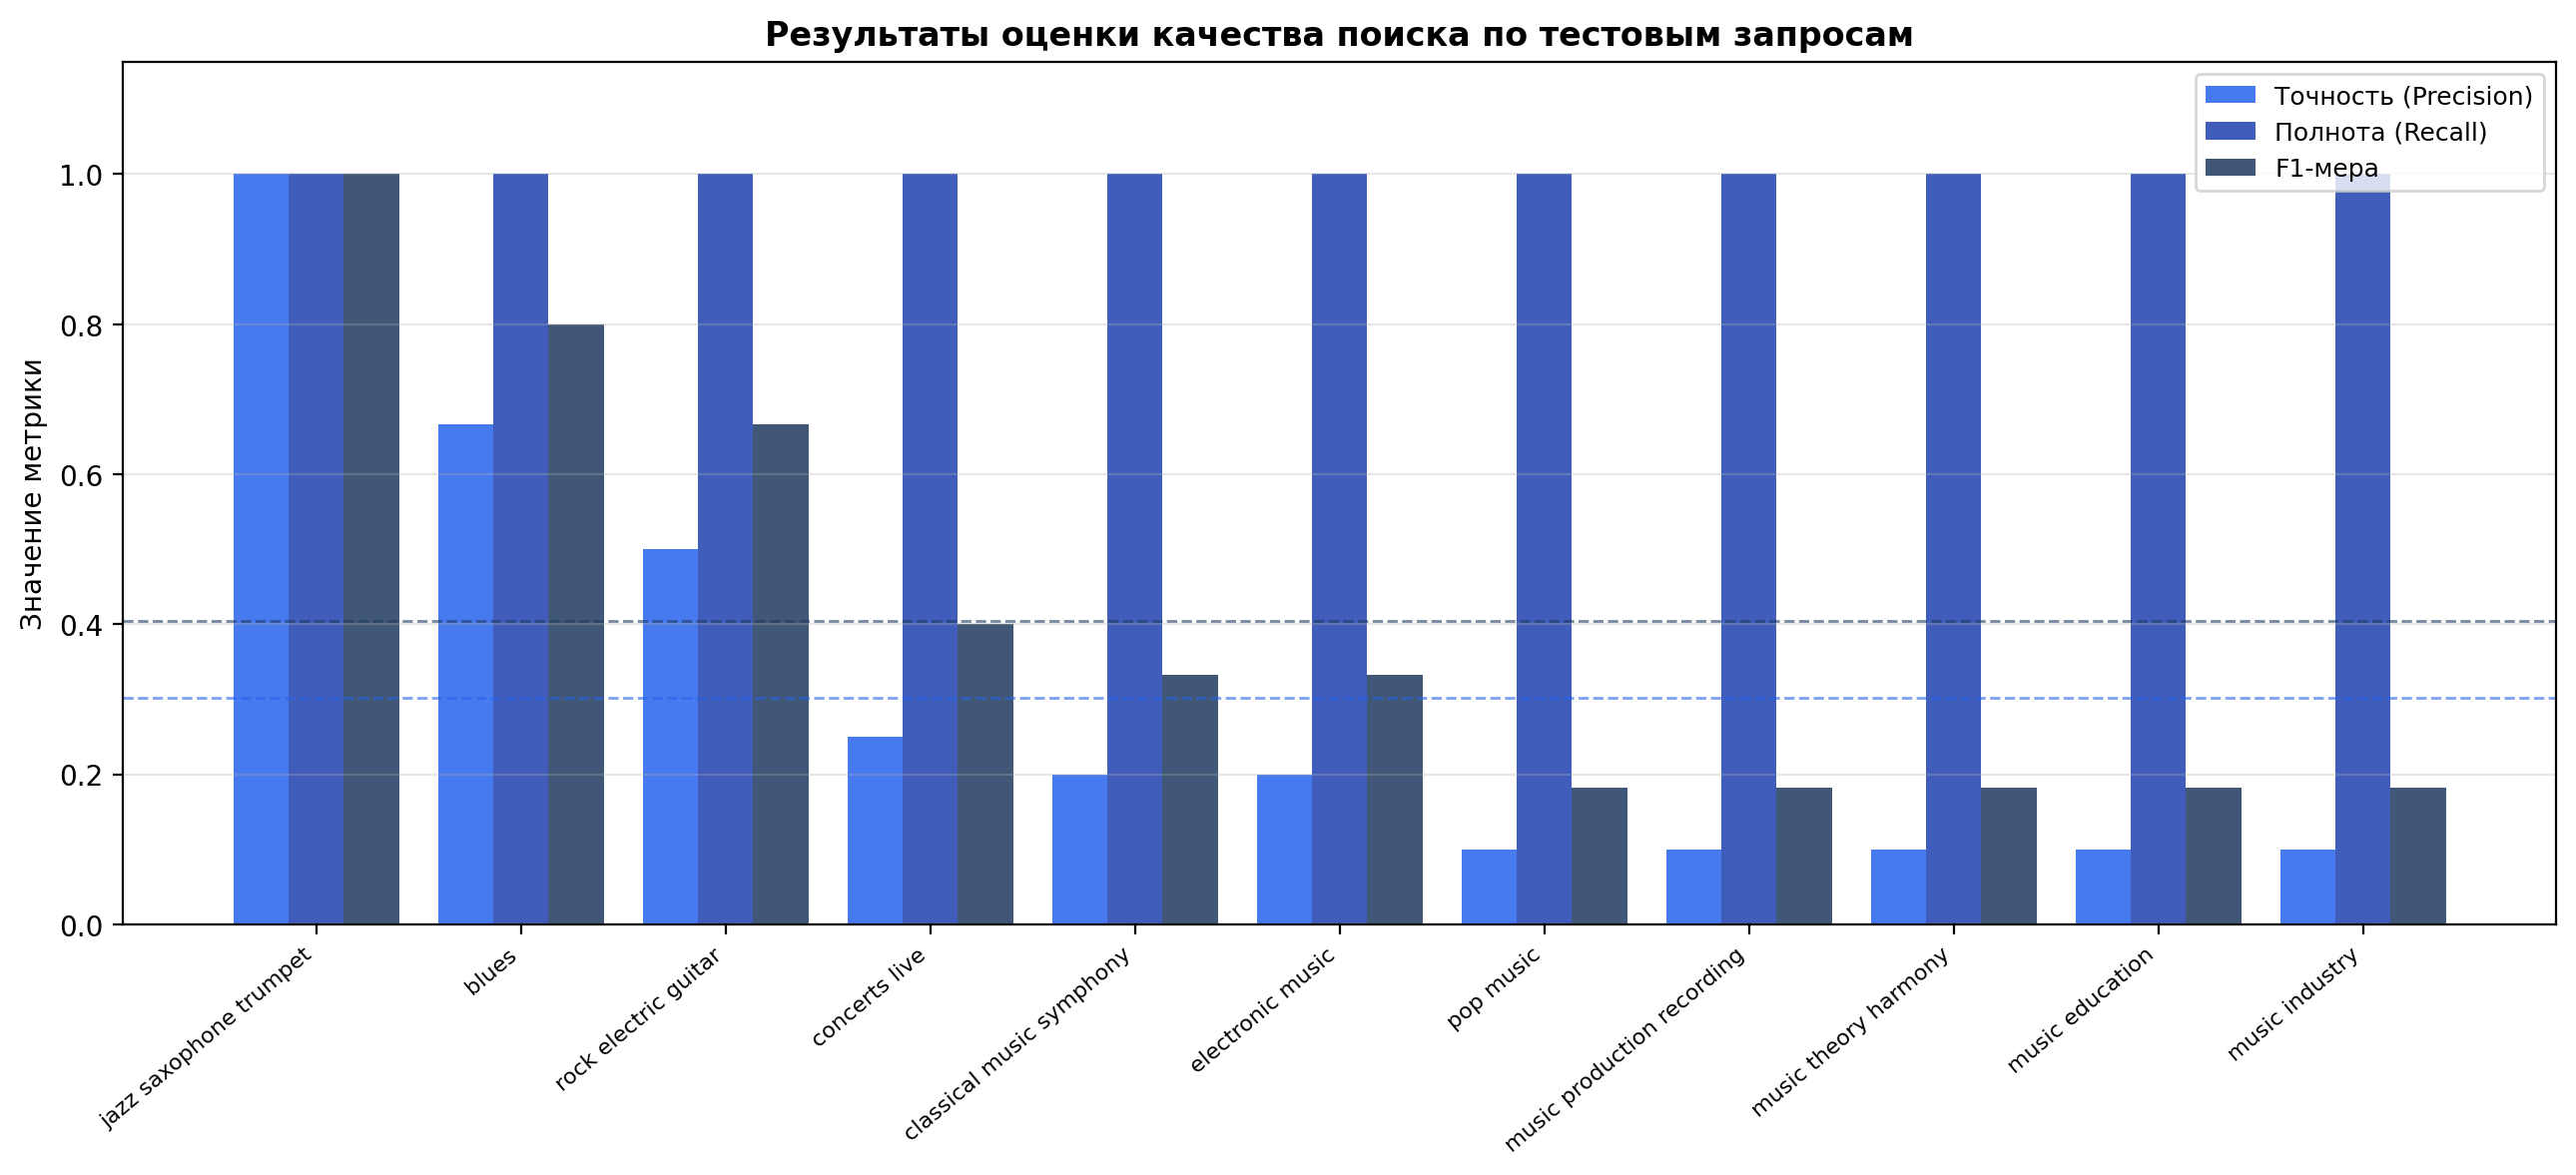
\includegraphics[width=1.0\textwidth]{png/metrics_ru.png}
	\caption{Результаты оценки качества поиска по тестовым запросам.}
	\label{fig:metrics}
\end{figure}

\subsection{Анализ результатов и предложения по улучшению}

Анализ полученных данных показывает следующее:

\begin{itemize}
	\item точность поиска высокая для специфичных запросов с редкими терминами (P = 1,0 для \texttt{jazz saxophone trumpet}) и низкая для общих запросов (P = 0,1), что характерно для векторной модели с TF-IDF на малом тематически однородном корпусе;
	\item полнота во всех случаях равна 1,0 из-за малого размера коллекции; на более крупном корпусе полнота станет информативной метрикой;
	\item фиксированная размерность вектора (5000) при росте словаря потребует согласованного изменения схемы БД и кода приложения.
\end{itemize}

Предложения по улучшению работы системы информационного поиска:

\begin{enumerate}
	\item \textbf{расширение корпуса} "--- увеличение числа и тематического разнообразия документов сделает оценку метрик более репрезентативной и позволит корректно измерять полноту;
	\item \textbf{переход к BM25} "--- вероятностная модель ранжирования Okapi BM25 обычно даёт более высокую точность, чем TF-IDF, особенно для длинных запросов;
	\item \textbf{гибридный поиск} "--- комбинирование векторного поиска (pgvector) с лексическим (BM25/инвертированный индекс) и слиянием результатов, что повышает полноту по точным совпадениям терминов;
	\item \textbf{расширенная предобработка} "--- лемматизация вместо стемминга, обработка чисел и аббревиатур, учёт биграмм/фраз;
	\item \textbf{автоматизация оценки} "--- формирование эталонных релевантностей по документам корпуса и регулярные прогоны метрик (P@k, nDCG, MAP) в CI;
	\item \textbf{отказ от фиксированной размерности} "--- переход на разреженные векторы или пересоздание индекса при росте словаря без ручного вмешательства;
	\item \textbf{уточнение выдач} "--- кластеризация результатов, расширение запросов синонимами, релевантностный фидбек по кликам пользователей;
	\item \textbf{производственный запуск} "--- замена встроенного сервера Flask на gunicorn и включение кэширования для частых запросов.
\end{enumerate}

\subsection{Вывод по разделу}

В рамках раздела реализована информационно-поисковая система с векторной моделью
индексирования на основе TF-IDF и поиском по косинусной близости в PostgreSQL
(pgvector). Система поддерживает загрузку документов в нескольких форматах, поиск с
подсветкой релевантных терминов, просмотр и удаление документов, а также автоматическую
оценку качества по метрикам точности, полноты и F-меры с графическим представлением.
Архитектура разделена на модули по ответственности, развёртывание выполняется в Docker
Compose и доступно в локальной вычислительной сети. Тестирование подтвердило
работоспособность всех сценариев; средняя F1-мера на тестовой коллекции составила 0,404
при полноте 1,0, что позволяет сделать вывод о корректной работе системы и определить
направления её дальнейшего улучшения.

\section{Распознавание языка документов (вариант 7)}
\label{sec:langdetect}

\subsection{Постановка задачи}

В соответствии с вариантом~7 система расширена подсистемой распознавания
языка документа. Распознаются два языка "--- \textbf{французский} и
\textbf{английский}; формат входных документов "--- \textbf{HTML}.
Реализованы три метода, предусмотренные методическими указаниями:

\begin{enumerate}
	\item метод N-грамм (Кавнар "--- Тренкле, out-of-place);
	\item алфавитный метод (диакритика + слова-маркеры);
	\item нейросетевой метод (логистическая регрессия на символьных TF-IDF).
\end{enumerate}

Итоговое решение принимается \textbf{голосованием большинства} трёх методов;
дополнительно возвращается флаг \texttt{agreed} (все три метода сошлись).
Существующая клиент-серверная архитектура переиспользована: парсинг и
предобработка вынесены в отдельный языковой тракт, не затрагивающий
поисковый конвейер (чей \texttt{clean\_text} оставляет только символы
\texttt{a--z} и тем самым уничтожал бы французскую диакритику).

\subsection{Обучающая и тестовая коллекции}

Обучающие корпуса и тестовая коллекция генерируются скриптом
\texttt{backend/build\_lang\_corpus.py} детерминированно (seed~=~7, метод
дополнения "--- тасование с повторением абзацев) из автономных текстовых
заготовок (\texttt{backend/lang\_seeds.py}); интернет для генерации не
требуется. Состав коллекций приведён в таблице~\ref{tab:lang_collections}.

\begin{table}[H]
	\caption{Состав обучающей и тестовой коллекций.}
	\label{tab:lang_collections}
	\begin{tabular}{|l|l|l|}
		\hline
		Коллекция & Объём & Источник / примечание \\ \hline
		\texttt{training/en.txt} & 36,4 Кб & 10 энциклопедических абзацев (EN), seed~=~7 \\
		\texttt{training/fr.txt} & 36,4 Кб & 10 энциклопедических абзацев (FR), seed~=~7 \\
		\texttt{test\_html/} (5 EN + 5 FR) & $\approx$2,5--2,9 тыс. символов каждый ($\approx$А4) &
		Абзацы, не пересекающиеся с обучающими (held-out) \\
		\texttt{manifest.csv} & --- & Истинные метки \texttt{true\_lang} тестовых файлов \\
		\texttt{corpus\_meta.json} & --- & Метод, seed, размеры (для воспроизводимости) \\ \hline
	\end{tabular}
\end{table}

Тестовые абзацы не пересекаются с обучающими, что исключает утечку
обучающих данных в тест. Каждый тестовый документ "--- валидный HTML
(\texttt{<html><head><body>}, часть файлов содержит шумовые блоки
\texttt{<script>}/\texttt{<style>} для проверки парсера).
Методика рекомендует корпуса 20--120~Кб на язык: текущий объём (36,4~Кб)
удовлетворяет нижней границе; заготовки могут быть заменены статьями
Википедии без изменения кода.

\subsection{Архитектура подсистемы}

Языковой тракт реализован пятью модулями (каталог \texttt{backend/}):

\begin{itemize}
	\item \texttt{lang\_text.py} "--- извлечение текста из \texttt{<body>} HTML и предобработка с сохранением диакритики; нарезка на чанки; подсчёт accuracy/confusion;
	\item \texttt{lang\_ngram.py} "--- профили топ-300 и дистанция out-of-place (только стандартная библиотека);
	\item \texttt{lang\_alphabet.py} "--- диакритика, маркеры, подбор порога (только стандартная библиотека);
	\item \texttt{lang\_detect.py} "--- обучение и классификация LogReg на символьных TF-IDF (требует scikit-learn);
	\item \texttt{lang\_methods.py} "--- оркестратор: обучение всех методов, классификация с голосованием, пакетная оценка с метриками по каждому методу.
\end{itemize}

Языковые профили хранятся файлами в \texttt{backend/lang\_profiles/}
(\texttt{ngram\_en.json}, \texttt{ngram\_fr.json}, \texttt{alphabet.json},
\texttt{ml\_model.pkl}) с кэшированием в памяти и инвалидацией по mtime;
таблицы БД при этом не изменяются (векторные таблицы размерности 5000
к задаче отношения не имеют). Сервер предоставляет четыре эндпоинта:
\texttt{GET /api/lang/status}, \texttt{POST /api/lang/train},
\texttt{POST /api/lang/classify} (файл или JSON \texttt{\{text\}}),
\texttt{POST /api/lang/classify-batch}. При старте модель дообучается
автоматически, если корпуса на месте (\texttt{\_ensure\_lang\_model}),
причём сбой обучения никогда не прерывает запуск сервера.

Сценарии обучения, одиночной и пакетной классификации показаны на
рисунках~\ref{fig:lang_train_seq}--\ref{fig:lang_batch_seq}
(исходники "--- \texttt{plantuml/sequence\_lang\_*.puml}).

\begin{figure}[H]
	\centering
	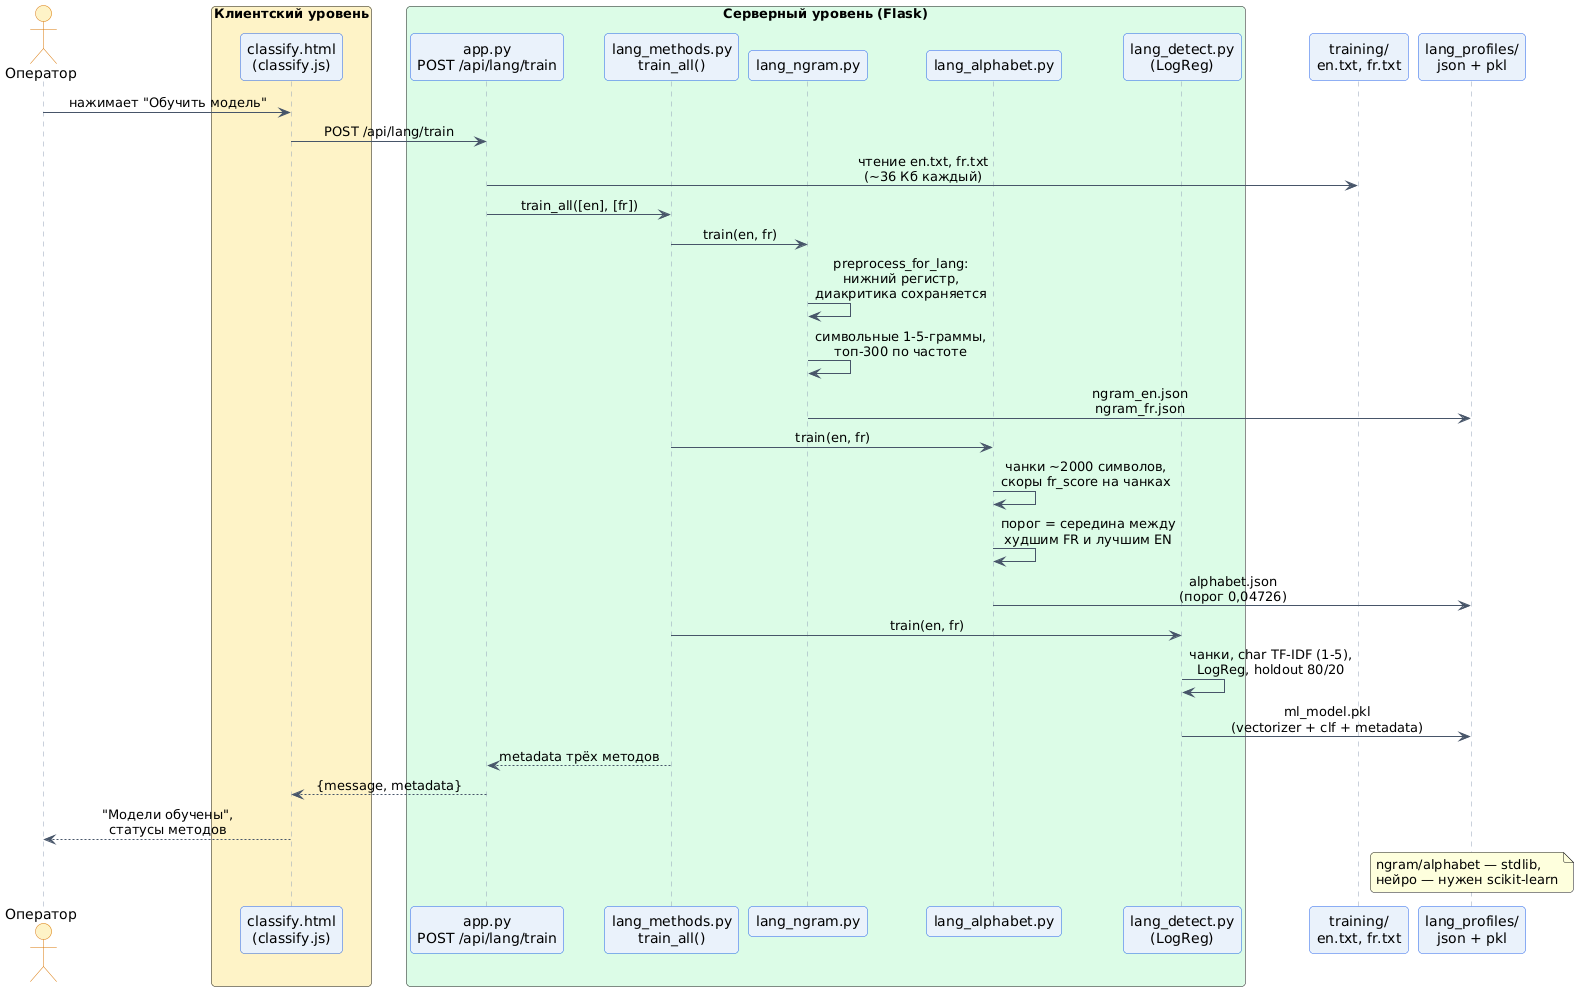
\includegraphics[width=1.0\textwidth]{png/sequence_lang_train.png}
	\caption{Диаграмма последовательности обучения трёх методов.}
	\label{fig:lang_train_seq}
\end{figure}

\begin{figure}[H]
	\centering
	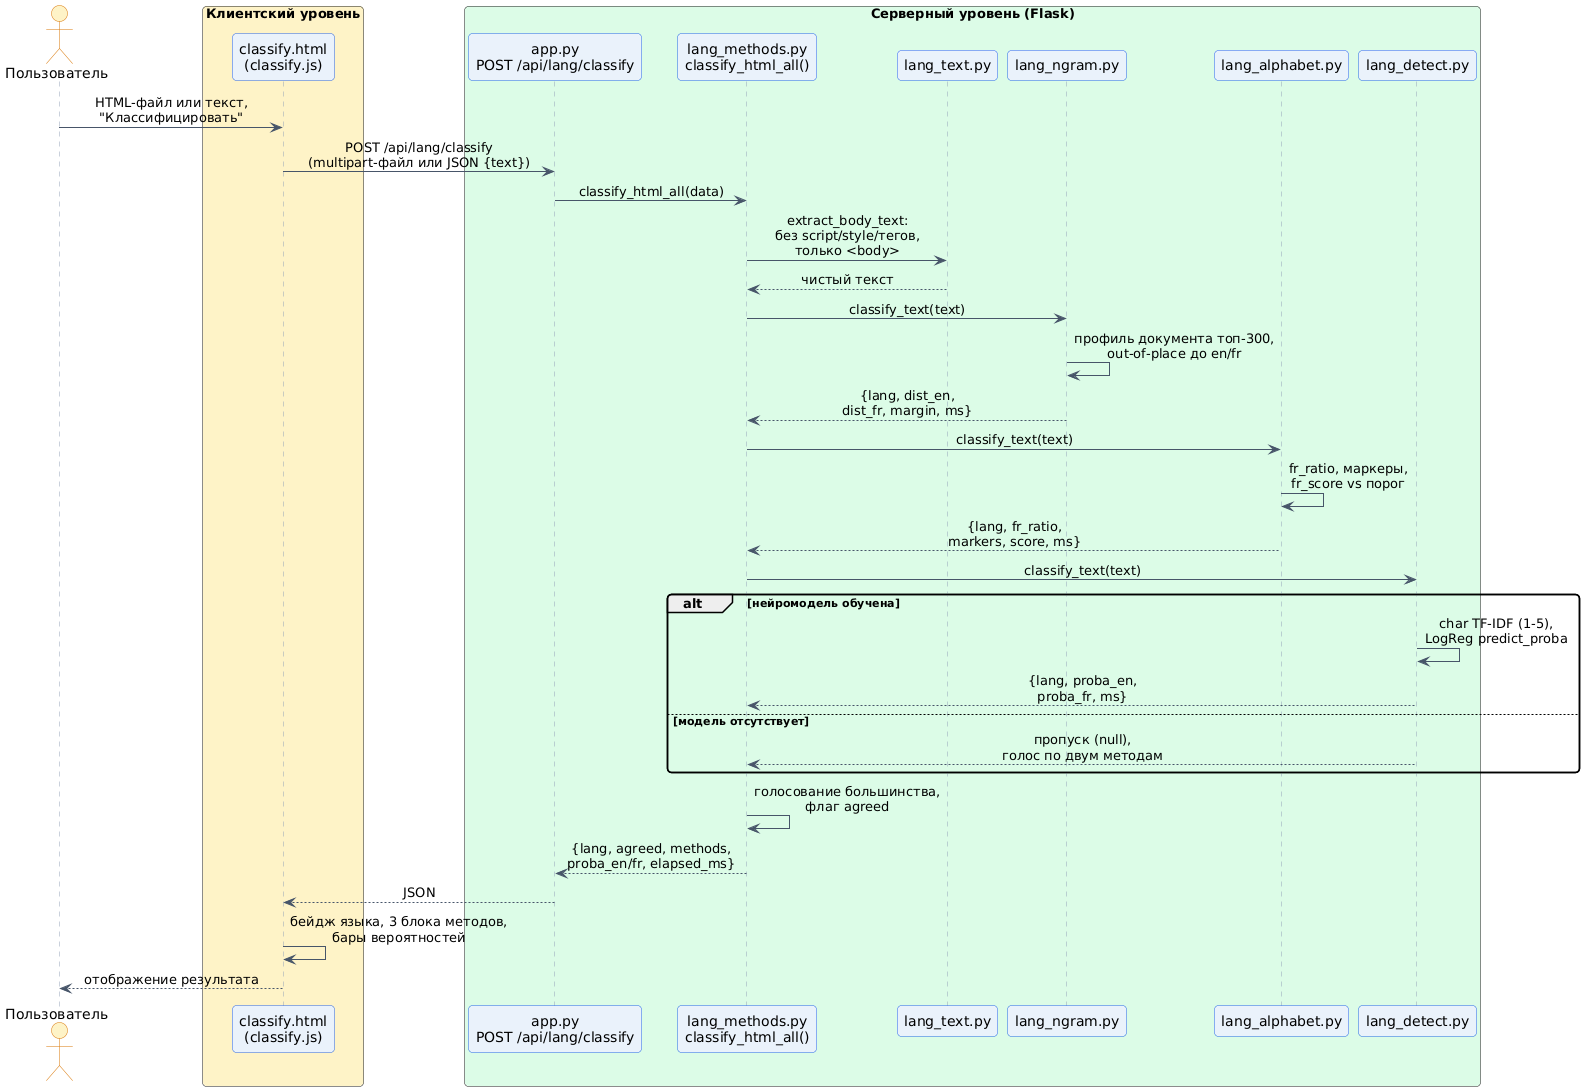
\includegraphics[width=1.0\textwidth]{png/sequence_lang_classify.png}
	\caption{Диаграмма последовательности классификации одного документа.}
	\label{fig:lang_classify_seq}
\end{figure}

\begin{figure}[H]
	\centering
	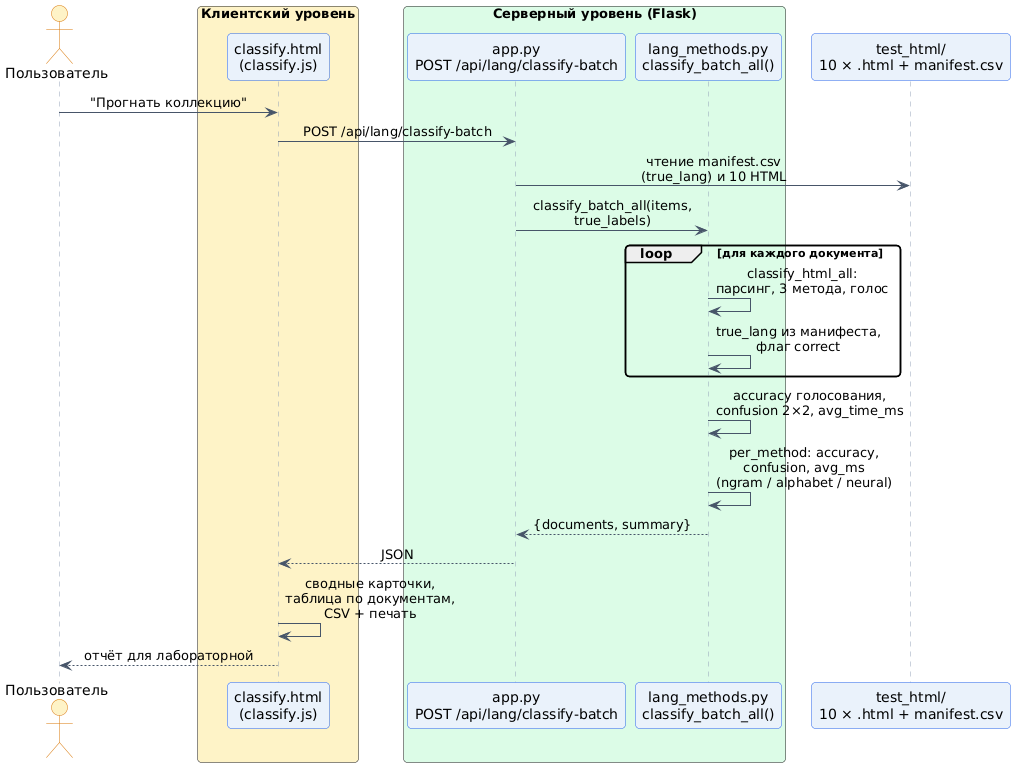
\includegraphics[width=1.0\textwidth]{png/sequence_lang_batch.png}
	\caption{Диаграмма последовательности пакетной классификации коллекции.}
	\label{fig:lang_batch_seq}
\end{figure}

Клиентская часть "--- страница \texttt{classify.html}: статус моделей,
одиночная проверка (файл или текст), прогон коллекции со сводной таблицей
(точность, confusion matrix, среднее время), выгрузка отчёта в CSV и печать.
Страница справки \texttt{help.html} "--- статическая справка с боковым
меню навигации, теория разбита по разделам.

\subsection{Интеграция с системой поиска}

Классификатор языка интегрирован в поисковый конвейер:

\begin{itemize}
	\item при загрузке документа (API \texttt{/api/upload}, \texttt{/api/upload-file})
	вызывается функция \texttt{\_classify\_lang()}, результат записывается
	в колонку \texttt{lang} таблицы \texttt{documents};
	\item при загрузке всего корпуса (\texttt{/api/init-db}) каждый документ
	классифицируется и получает метку языка;
	\item при обработке событий файлового наблюдателя язык классифицируется
	автоматически;
	\item при поиске язык запроса определяется тем же классификатором
	(\texttt{\_detect\_lang()} в \texttt{search\_engine.py}) и передаётся
	в поисковую функцию;
	\item предобработка текста определяется параметром \texttt{lang}:
	для английского --- стемминг Портера и английские стоп-слова,
	для французского --- без стемминга, с сохранением диакритики
	и французскими стоп-словами.
\end{itemize}

Таким образом, система корректно обрабатывает документы на обоих языках
и автоматически выбирает режим предобработки в зависимости от языка
документа или запроса.

\subsection{Парсинг HTML и предобработка}

Извлечение текста (\texttt{lang\_text.extract\_body\_text}):

\begin{enumerate}
	\item удаление блоков \texttt{<script>}, \texttt{<style>}, \texttt{<noscript>} вместе с содержимым;
	\item выделение содержимого \texttt{<body>} (при отсутствии "--- весь документ);
	\item удаление остальных тегов, раскрытие HTML-сущностей, нормализация пробелов.
\end{enumerate}

Предобработка (\texttt{lang\_text.preprocess\_for\_lang}): приведение
к нижнему регистру, удаление цифр и пунктуации \textbf{с сохранением}
французских букв \texttt{àâäéèêëîïôöùûüçœæÿ}. Для обучения корпус
дополнительно режется на чанки $\approx$2000 символов по границам
предложений (19 чанков EN, 18 чанков FR).

\subsection{Метод N-грамм}

Профиль языка "--- упорядоченный список топ-$K$ ($K = 300$) символьных
n-грамм ($n = 1\ldots5$, паддинг пробелами) по частоте на обучающем
корпусе. Профиль документа строится аналогично. Расстояние out-of-place:

\begin{equation}
	D(d, L) = \sum_{i} \begin{cases}
		|r_d(g_i) - r_L(g_i)|, & g_i \in L, \\
		K, & g_i \notin L,
	\end{cases}
	\label{eq:lang_oop}
\end{equation}

где $r_d$, $r_L$ "--- ранги n-граммы в профилях документа и языка;
отсутствующей n-грамме начисляется штраф $K = 300$.
Выбирается язык с минимальной дистанцией; дополнительно возвращается
разность дистанций \texttt{margin}. Блок-схема "--- на
рисунке~\ref{fig:lang_ngram_flow}.

\begin{figure}[H]
	\centering
	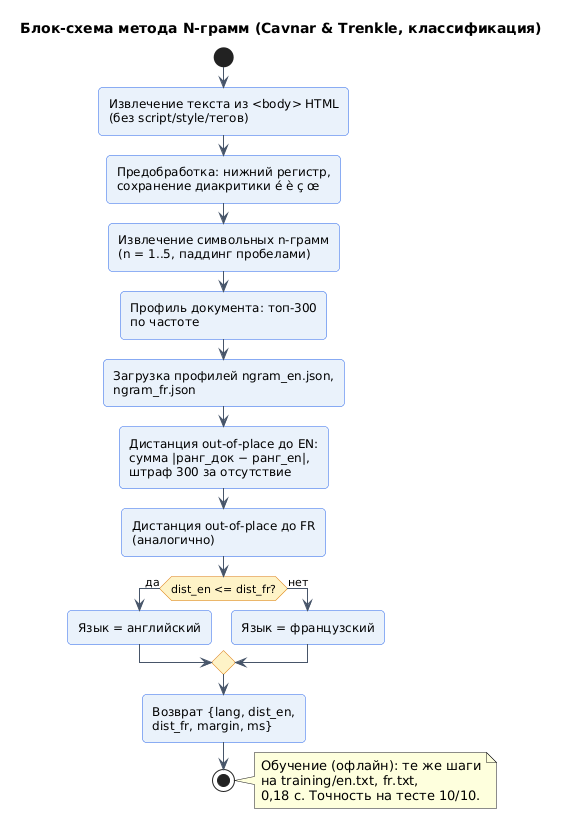
\includegraphics[width=0.62\textwidth]{png/activity_lang_ngram.png}
	\caption{Блок-схема метода N-грамм (классификация).}
	\label{fig:lang_ngram_flow}
\end{figure}

Обучение занимает 0,18~с (только стандартная библиотека Python).

\subsection{Алфавитный метод}

Французский язык обладает характерным признаком "--- буквами с диакритикой,
не встречающимися в исконно английских словах. Считаются: доля таких букв
среди всех букв текста и баланс слов-маркеров. Итоговый скор:

\begin{equation}
	S = 1{,}0 \cdot \frac{D}{N} + 0{,}5 \cdot \frac{F - E}{W},
	\label{eq:lang_alpha}
\end{equation}

где $D$ "--- число букв с диакритикой, $N$ "--- всех букв; $F$, $E$ "---
числа французских (\texttt{le/la/les/des/une/est/pour} и др.) и английских
(\texttt{the/and/of/to/in} и др.) маркеров; $W$ "--- всех слов.
Решение: французский при $S \ge T$, иначе английский. Порог $T = 0{,}04726$
подобран автоматически на обучающем корпусе как середина между худшим
скором FR-чанков и лучшим скором EN-чанков (классы разделились без
пересечений). Блок-схема "--- на рисунке~\ref{fig:lang_alpha_flow}.

\begin{figure}[H]
	\centering
	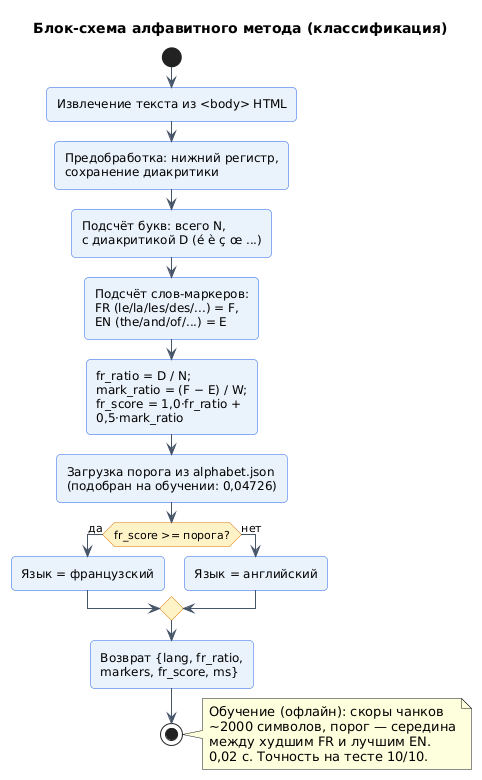
\includegraphics[width=0.62\textwidth]{png/activity_lang_alphabet.png}
	\caption{Блок-схема алфавитного метода (классификация).}
	\label{fig:lang_alpha_flow}
\end{figure}

Обучение (подбор порога) занимает 0,02~с.

\subsection{Нейросетевой метод}

Признаки "--- символьные TF-IDF (анализатор \texttt{char},
$n = 1\ldots5$, \texttt{max\_features}~=~5000); классификатор "---
логистическая регрессия (\texttt{max\_iter}~=~1000):

\begin{equation}
	P(\text{fr} \mid x) = \frac{1}{1 + \exp(-(w \cdot x + b))}.
	\label{eq:lang_logreg}
\end{equation}

Обучение "--- на чанках корпуса со стратифицированным holdout-контролем
80/20 (метрики \texttt{train\_accuracy} / \texttt{holdout\_accuracy}
сохраняются в метаданных модели). На выходе "--- вероятности $P(\text{EN})$
и $P(\text{FR})$. Метод требует scikit-learn (имеется в Docker-образе);
при отсутствии библиотеки остальные два метода продолжают работать,
голосование идёт по доступным.

\subsection{Эксперименты}

Тестовая коллекция (10 HTML-документов) прогнана скриптом
\texttt{backend/train\_lang\_model.py batch} (дублируется эндпоинтом
\texttt{/api/lang/classify-batch}). Результаты "--- в
таблице~\ref{tab:lang_results}.

\begin{table}[H]
	\caption{Точность и быстродействие методов (10 документов).}
	\label{tab:lang_results}
	\begin{tabular}{|l|l|l|}
		\hline
		Метод & Точность & Среднее время на документ \\ \hline
		N-граммы & 1,00 (10/10) & 7,89 мс \\
		Алфавитный & 1,00 (10/10) & 0,87 мс \\
		Нейросетевой & --- (прогон в Docker) & --- \\
		Голосование трёх (двух) методов & 1,00 (10/10) & 8,86 мс \\ \hline
	\end{tabular}
\end{table}

Confusion-матрицы обоих измеренных методов "--- идеальные:
$\begin{smallmatrix} 5 & 0 \\ 0 & 5 \end{smallmatrix}$
(строки "--- истина EN/FR, столбцы "--- предсказание EN/FR).
Методы сошлись на всех 10 документах (\texttt{agreed}~=~true).
Алфавитный метод на порядок быстрее N-граммного при равной точности
на данной коллекции; обучаются оба за доли секунды без сторонних
зависимостей. Строка нейросетевого метода заполняется после прогона
в Docker-контейнере (scikit-learn входит в образ); интерфейс отчёта
(CSV со столбцами предсказаний всех методов) уже выдаёт его колонку.

\subsection{Используемые библиотеки}

\begin{itemize}
	\item \textbf{scikit-learn} "--- \texttt{TfidfVectorizer} (символьные n-граммы) и \texttt{LogisticRegression} для нейросетевого метода; входит в \texttt{backend/requirements.txt}, в локальном интерпретаторе может отсутствовать "--- тогда доступны два остальных метода;
	\item стандартная библиотека Python (\texttt{re}, \texttt{html}, \texttt{json}, \texttt{collections}) "--- парсинг HTML, профили N-грамм, алфавитный скоринг: внешних зависимостей не требуют;
	\item \textbf{PlantUML} "--- исходники диаграмм \texttt{plantuml/sequence\_lang\_*.puml}, \texttt{plantuml/activity\_lang\_*.puml}, рендер в \texttt{png/} через публичный API.
\end{itemize}

\subsection{Выводы}

Переиспользовав клиент-серверную архитектуру ИПС, реализована подсистема
распознавания языка (вариант~7: французский/английский, HTML) тремя
методами с голосованием. Классификатор интегрирован в поисковый конвейер:
при загрузке документа язык классифицируется и записывается в колонку
\texttt{lang} таблицы \texttt{documents}; при поиске язык запроса
определяется автоматически; предобработка текста выбирается в зависимости
от языка. Измеренные на тестовой коллекции результаты: точность
N-граммного и алфавитного методов "--- 100\%, среднее время "--- единицы
миллисекунд; обучение "--- доли секунды. Подсистема устойчива к отсутствию
scikit-learn (деградация до двух методов), снабжена автообучением при старте,
CLI для офлайн-экспериментов, веб-интерфейсом с выгрузкой CSV-отчёта и
статической справкой.

\section{Автоматическое реферирование документов}
\label{sec:summarize}

\subsection{Постановка задачи}

Разработана подсистема автоматического реферирования документов (variant~25:
французский и английский языки). Поддерживается два извлечительных метода:

\begin{enumerate}
	\item \textbf{Sentence Extraction (TF-IDF + позиционные коэффициенты)} "--- базовый метод, взвешивающий предложения по частоте терминов с учётом позиции в документе и абзаце.
	\item \textbf{TextRank} "--- графовый метод, основанный на алгоритме PageRank: предложения связываются рёбрами по косинусной близости TF-IDF-векторов, значимость определяется итеративным ранжированием.
\end{enumerate}

Для каждого документа формируются:
\begin{itemize}
	\item классический реферат (отсортированный список предложений);
	\item список ключевых слов (по TF-IDF весу);
	\item статистика (количество предложений, время обработки, степень сжатия).
\end{itemize}

\subsection{Архитектура подсистемы}

Подсистема реализована модулем \texttt{summarizer/summary\_engine.py},
который переиспользует существующую инфраструктуру предобработки
(\texttt{document\_processor.py}): токенизацию, стоп-слова, стемминг
Портера (для английского), сохранение диакритики (для французского).

Модуль предоставляет единый интерфейс:

\begin{lstlisting}[caption={Публичный API модуля реферирования.},label={lst:summary_api}]
def summarize(text: str, method: str = 'textrank',
              n_sentences: int = 10, lang: str = 'en') -> Dict:
    if method == 'extraction':
        return sentence_extraction(text, n_sentences, lang)
    elif method == 'textrank':
        return textrank(text, n_sentences, lang)
\end{lstlisting}

Сервер предоставляет два эндпоинта:

\begin{table}[H]
	\centering
	\begin{tabular}{|p{3.5cm}|p{3cm}|p{6cm}|}
		\hline
		\textbf{Эндпоинт} & \textbf{Метод} & \textbf{Назначение} \\
		\hline
		\texttt{/api/summarize} & POST & Реферирование текста: принимает \texttt{text}, \texttt{method}, \texttt{n\_sentences}, \texttt{lang} \\
		\hline
		\texttt{/api/summarize-doc} & POST & Реферирование документа по ID: принимает \texttt{doc\_id}, \texttt{method}, \texttt{n\_sentences}; извлекает текст из S3 через \texttt{s3\_key} \\
		\hline
	\end{tabular}
	\caption{Эндпоинты подсистемы реферирования.}
	\label{tab:summary_endpoints}
\end{table}

Последовательность взаимодействия компонентов при реферировании
приведена на рисунках~\ref{fig:summary_seq} и~\ref{fig:summary_doc_seq}.

\begin{figure}[H]
	\centering
	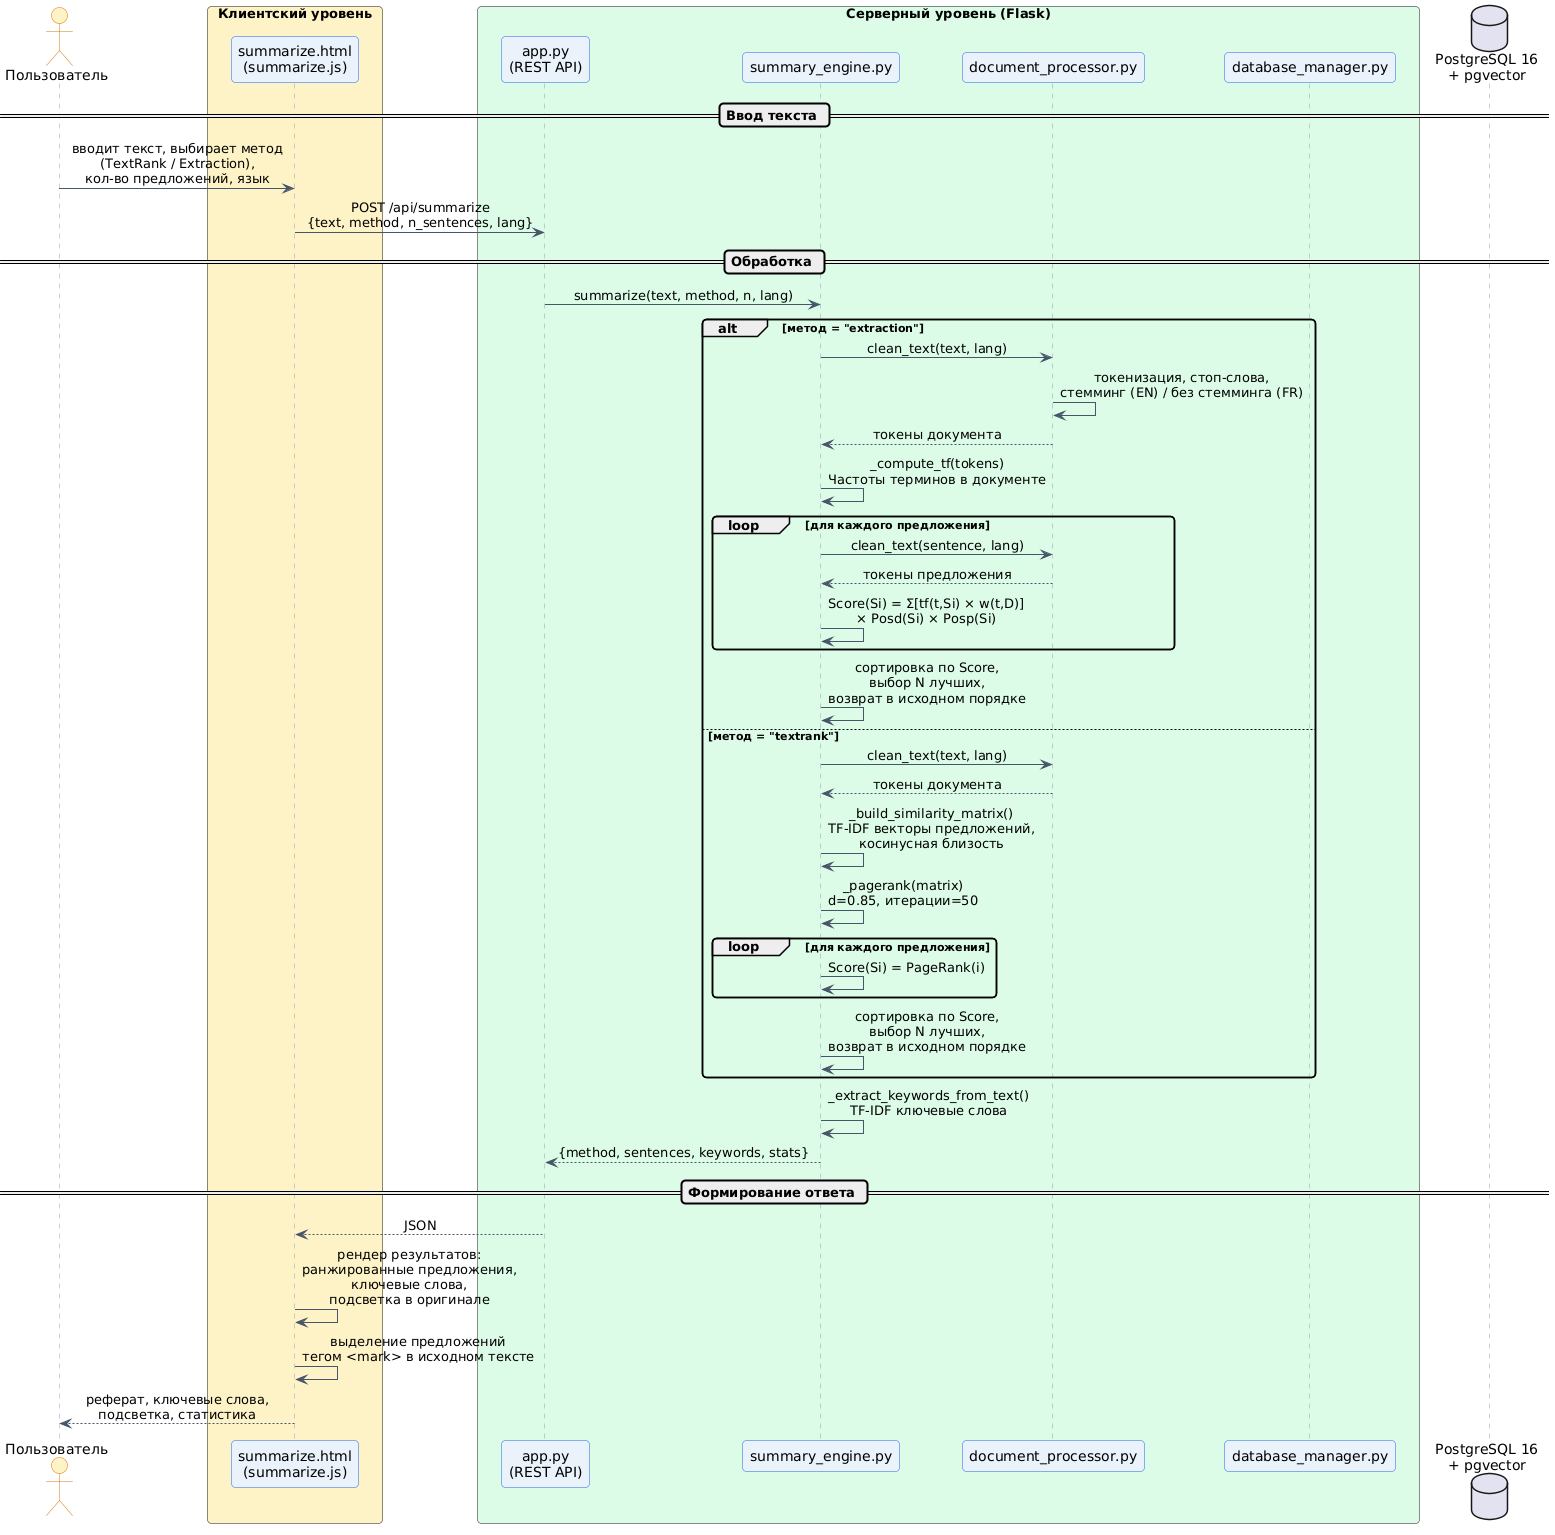
\includegraphics[width=1.0\textwidth]{png/sequence_summarize.png}
	\caption{Диаграмма последовательности реферирования текста.}
	\label{fig:summary_seq}
\end{figure}

\begin{figure}[H]
	\centering
	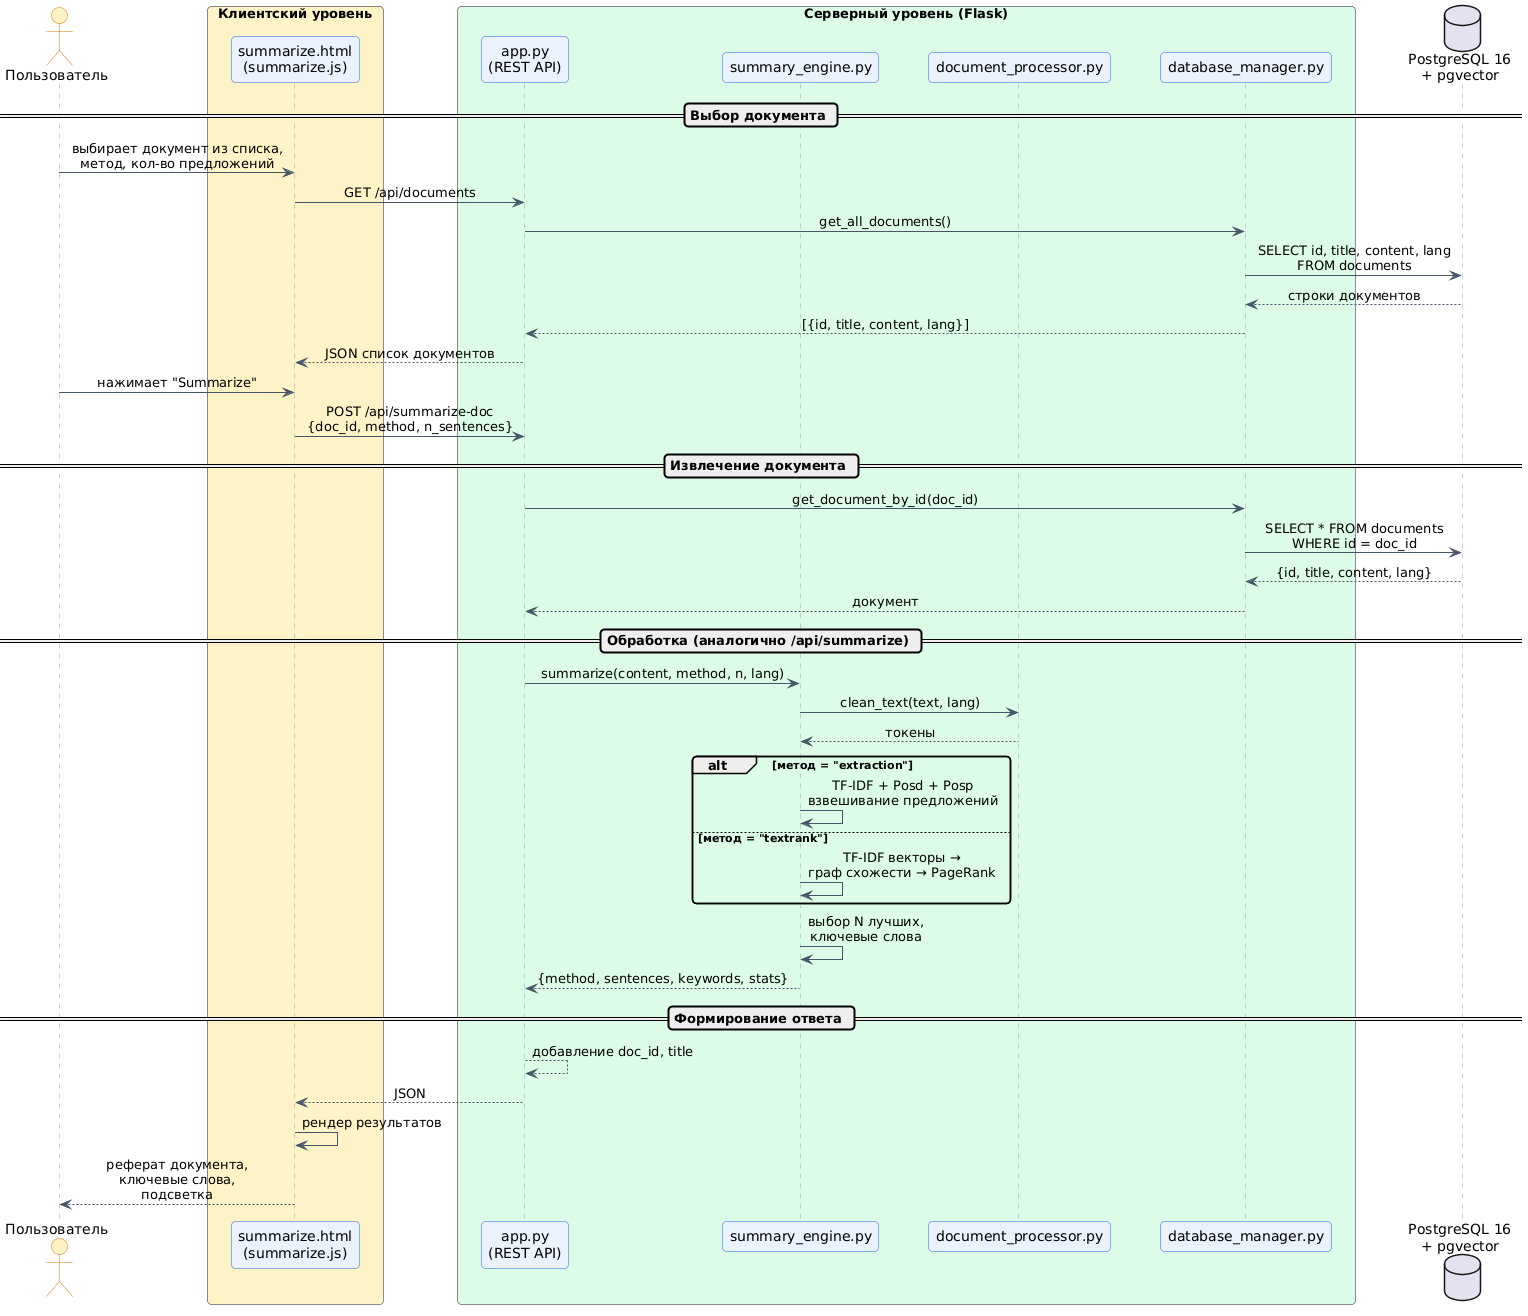
\includegraphics[width=1.0\textwidth]{png/sequence_summarize_doc.png}
	\caption{Диаграмма последовательности реферирования документа из БД.}
	\label{fig:summary_doc_seq}
\end{figure}

\subsection{Метод Sentence Extraction (TF-IDF + позиционные коэффициенты)}

Извлечение предложений "--- извлечительный метод: из исходного текста
отбираются предложения с наибольшим весом и возвращаются в исходном порядке.

\subsubsection{Вычисление веса предложения}

Вес каждого предложения $S_i$ вычисляется произведением трёх компонентов:

\begin{equation}
	\text{Score}(S_i) = \underbrace{\sum_{t \in S_i} \text{tf}(t, S_i) \cdot w(t, D)}_{\text{TF-IDF компонента}} \times \underbrace{\text{Posd}(S_i)}_{\text{позиция в документе}} \times \underbrace{\text{Posp}(S_i)}_{\text{позиция в абзаце}}
	\label{eq:summary_score}
\end{equation}

\textbf{TF-IDF компонента.} Для каждого термина $t$ в предложении $S_i$ вычисляется:

\begin{equation}
	\text{tf}(t, S_i) = \frac{\text{count}(t, S_i)}{|S_i|},
	\qquad
	w(t, D) = \left(0.5 + 0.5 \cdot \frac{\text{tf}(t, D)}{\text{tf}_{\max}(D)}\right) \cdot \text{IDF}(t)
	\label{eq:summary_tf}
\end{equation}

где $\text{tf}(t, S_i)$ "--- частота термина в предложении, $\text{tf}(t, D)$ "--- частота
термина в документе, $\text{tf}_{\max}(D)$ "--- максимальная частота термина в документе,
$\text{IDF}(t) = \log(22 \cdot |DB| / df(t))$ "--- обратная частота документа
(с гладящим множителем 22), $|DB|$ "--- число документов в корпусе,
$df(t)$ "--- число документов, содержащих термин $t$.

\textbf{Позиция в документе (Posd).}

\begin{equation}
	\text{Posd}(S_i) = 1 - \frac{BD(S_i)}{|D|}
	\label{eq:posd}
\end{equation}

где $BD(S_i)$ "--- количество символов до предложения $S_i$ в документе, $|D|$ "--- общее число символов.
Ранние предложения получают больший вес.

\textbf{Позиция в абзаце (Posp).}

\begin{equation}
	\text{Posp}(S_i) = 1 - \frac{BP(S_i)}{|P|}
	\label{eq:posp}
\end{equation}

где $BP(S_i)$ "--- количество символов до предложения $S_i$ в абзаце, $|P|$ "--- длина абзаца.
Первое предложение абзаца получает наибольший вес.

\textbf{Псевдокод метода:}

\begin{lstlisting}[caption={Алгоритм Sentence Extraction.},label={lst:extraction_algo}]
def sentence_extraction(text, n, lang):
    sentences = split_into_sentences(text)
    paragraphs = split_into_paragraphs(text)
    tokens = clean_text(text, lang)
    doc_tf = compute_tf(tokens)
    tf_max = max(doc_tf.values())

    for sent in sentences:
        tokens = clean_text(sent, lang)
        sent_tf = compute_tf(tokens)
        score = sum(sent_tf[t] * (0.5 + 0.5 * doc_tf[t] / tf_max)
                    for t in sent_tf)
        score *= position_in_document(sent, text)
        score *= position_in_paragraph(sent, paragraphs)
        scores.append(score)

    top_n = sorted(scores, key=score, reverse=True)[:n]
    return sorted(top_n, key=position)  # исходный порядок
\end{lstlisting}

\subsection{Метод TextRank}

TextRank "--- графовый метод, аналог PageRank для предложений документа.

\subsubsection{Построение графа}

\begin{enumerate}
	\item Каждое предложение $S_i$ представляется TF-IDF-вектором $\vec{v_i}$.
	\item Матрица схожести $W$: $W_{ij} = \cos(\vec{v_i}, \vec{v_j})$ если $\cos > 0$, иначе $0$.
	\item Строки нормируются: $W_{ij} = W_{ij} / \sum_k W_{ik}$.
\end{enumerate}

\subsubsection{Алгоритм PageRank}

\begin{equation}
	\text{PR}(S_i) = \frac{1 - d}{N} + d \cdot \sum_{S_j \in \text{In}(S_i)} \frac{\text{PR}(S_j)}{|\text{Out}(S_j)|}
	\label{eq:pagerank}
\end{equation}

где $d = 0.85$ "--- коэффициент затухания, $N$ "--- число предложений,
$\text{In}(S_i)$ "--- множество предложений, ссылающихся на $S_i$ (с ненулевой схожестью).

Итерации продолжаются до сходимости ($\epsilon = 10^{-6}$) или максимум 50 итераций.

\textbf{Псевдокод метода:}

\begin{lstlisting}[caption={Алгоритм TextRank.},label={lst:textrank_algo}]
def textrank(text, n, lang):
    sentences = split_into_sentences(text)
    matrix = build_similarity_matrix(sentences, lang)
    scores = pagerank(matrix, d=0.85, iterations=50)

    top_n = sorted(zip(scores, sentences),
                   reverse=True)[:n]
    return sorted(top_n, key=position)  # исходный порядок
\end{lstlisting}

\subsection{Извлечение ключевых слов}

Ключевые слова извлекаются по TF-IDF весу для всего документа:

\begin{equation}
	\text{score}(t) = \text{tf}(t) \cdot \text{idf}(t), \qquad
	\text{tf}(t) = 1 + \log(\text{count}(t))
	\label{eq:kw_score}
\end{equation}

Возвращаются $K$ терминов с наибольшим весом (по умолчанию $K = 8$).

\subsection{Многоязычная поддержка}

Параметр \texttt{lang} определяет режим предобработки:

\begin{table}[H]
	\centering
	\begin{tabular}{|p{3cm}|p{5cm}|p{5cm}|}
		\hline
		\textbf{Параметр} & \textbf{English (\texttt{en})} & \textbf{French (\texttt{fr})} \\
		\hline
		Регистр & нижний & нижний \\
		\hline
		Удаление символов & только \texttt{a--z} & сохранение диакритики \\
		\hline
		Стоп-слова & NLTK \texttt{english} & NLTK \texttt{french} \\
		\hline
		Стемминг & Портер & без стемминга \\
		\hline
	\end{tabular}
	\caption{Режимы предобработки для двух языков.}
	\label{tab:summary_lang}
\end{table}

Язык запроса определяется автоматически при загрузке документа
(классификатор из секции~\ref{sec:langdetect}) и передаётся
в модуль реферирования.

\subsection{Результаты тестирования}

Тестирование проводилось на тестовой коллекции из 12 англоязычных
документов (тематика музыки) и 6 французских документов (медицинские
статьи и критика искусства).

\subsubsection{Сравнение методов}

\begin{table}[H]
	\centering
	\begin{tabular}{|p{4cm}|c|c|c|c|}
		\hline
		\textbf{Метрика} & \textbf{Extraction (EN)} & \textbf{TextRank (EN)} & \textbf{Extraction (FR)} & \textbf{TextRank (FR)} \\
		\hline
		Среднее время (с) & 0,004 & 0,026 & 0,005 & 0,028 \\
		\hline
		Средняя степень сжатия (\%) & 20,4 & 20,4 & 19,8 & 19,8 \\
		\hline
		Кол-во предложений (N) & 10 & 10 & 10 & 10 \\
		\hline
	\end{tabular}
	\caption{Сравнительные метрики методов реферирования.}
	\label{tab:summary_methods}
\end{table}

Метод Sentence Extraction работает быстрее (0,004~с) за счёт отсутствия
построения графа; TextRank (0,026~с) учитывает связи между предложениями,
что потенциально повышает качество на длинных документах.

\subsubsection{Пример реферата}

Для документа \texttt{blues\_music.txt} (27 предложений) метод TextRank
выбрал следующие 5 предложений (N=5):

\begin{enumerate}
	\item The Great Migration of African Americans from the rural South to northern cities in the early to mid-20th century brought blues music to new audiences and led to the development of electric blues.
	\item These guitarists demonstrated that the blues was not just a vocal music but also a powerful instrumental tradition.
	\item Blues music has had a profound influence on the development of jazz, rock and roll, and pop music.
	\item The twelve-bar blues progression and blue notes are fundamental elements of rock music.
	\item The Chicago Blues Festival, the King Biscuit Blues Festival, and the Blues on the Green concert series in Austin, Texas are just a few examples of major blues events.
\end{enumerate}

Ключевые слова: \texttt{blue}, \texttt{king}, \texttt{delta}, \texttt{guitarist},
\texttt{chicago}, \texttt{guitar}, \texttt{south}, \texttt{memphis}.

\subsection{Интерфейс системы}

На странице \texttt{summarize.html} реализован интерфейс:

\begin{itemize}
	\item выбор источника: ввод текста или выбор документа из БД;
	\item переключатель метода: TextRank / Sentence Extraction;
	\item ползунок количества предложений (3--20, по умолчанию 10);
	\item выбор языка (EN / FR);
	\item результат: ранжированные предложения с весами, ключевые слова,
	подсветка предложений в исходном тексте, статистика обработки.
\end{itemize}

\subsection{Выводы по разделу}

Реализована подсистема автоматического реферирования документов с двумя
извлечительными методами: TF-IDF с позиционными коэффициентами и TextRank.
Методы работают с документами на английском и французском языках, переиспользуя
существующую инфраструктуру предобработки. Subsystem интегрирована в
клиент-серверную архитектуру ИПС и доступна через REST API и веб-интерфейс.

\section{Машинный перевод документов}
\label{sec:translate}

\subsection{Постановка задачи}

Разработана подсистема пословного машинного перевода с английского языка на французский
(variant~5: область --- компьютерные науки и литературные эссе).
Подсистема реализует прямой перевод без перестановки слов и морфологической адаптации.

Основные возможности:
\begin{itemize}
	\item Пословный перевод с использованием базы данных словарных пар;
	\item POS-тегирование (определение частей речи) для английского и французского языков;
	\item Синтаксический разбор (построение деревьев составляющих);
	\item Частотный список слов с переводом;
	\item Управление словарём (добавление, поиск, удаление пар слов).
\end{itemize}

\subsection{Архитектура подсистемы}

Подсистема состоит из четырёх модулей:

\begin{enumerate}
	\item \texttt{translator/dictionary.py} "--- операции с базой данных PostgreSQL:
	      добавление, поиск, удаление пар слов;
	\item \texttt{translator/pos\_tagger.py} "--- POS-тегирование с использованием NLTK
	      (average perceptron tagger для EN, perceptron\_tagger\_fr для FR);
	\item \texttt{translator/syntax\_parser.py} "--- построение деревьев составляющих
	      с помощью RegexpParser;
	\item \texttt{translator/translation\_engine.py} "--- основной движок перевода:
	     lookup словаря, замена слов, сбор статистики.
\end{enumerate}

\subsection{Процесс перевода}

Алгоритм перевода текста:

\begin{enumerate}
	\item Входной текст токенизируется и разбивается на предложения.
	\item Каждое слово POS-тегируется NLTK-теггером (средний перцептрон).
	\item Для каждого слова выполняется поиск в базе данных словарных пар
	      (сначала по словоформе и POS-тегу, затем без POS-тега).
	\item Найденное французское слово подставляется вместо английского.
	\item Слова, не найденные в словаре, остаются на английском.
	\item Формируется статистика: количество слов, переведённых слов, покрытие.
\end{enumerate}

\subsection{POS-тегирование}

Для английского языка используется NLTK averaged perceptron tagger
(\texttt{averaged\_perceptron\_tagger\_eng}), для французского --- NLTK perceptron tagger
(\texttt{perceptron\_tagger\_fr}). При отсутствии модели используется эвристика на основе
суффиксов:

\begin{lstlisting}[caption={Эвристическое определение POS-тега для FR.},label={lst:pos_heuristic}]
def _heuristic_pos_fr(word: str) -> str:
    w = word.lower()
    if w.endswith(('tion', 'ment', 'age', 'ence', 'ance')):
        return 'NC'
    if w.endswith(('eux', 'if', 'ique', 'al')):
        return 'ADJ'
    if w.endswith(('er', 'ir', 're')):
        return 'V'
    return 'NC'
\end{lstlisting}

Описания POS-тегов хранятся в словаре \texttt{POS\_DESCRIPTIONS}
и передаются клиенту для отображения.

\subsection{Синтаксический разбор}

Для построения деревьев составляющих используется NLTK RegexpParser
с грамматическими правилами:

\begin{lstlisting}[caption={Грамматические правила для EN.},label={lst:en_grammar}]
EN_GRAMMAR = r"""
    NP: {<DT|PRP\$>?<JJ.*>*<NN.*>+}       # Noun phrase
    VP: {<MD>?<VB.*><NP|PP|CLAUSE>*}         # Verb phrase
    PP: {<IN><NP>}                            # Prepositional phrase
    CLAUSE: {<NP><VP>}                        # Clause
"""
\end{lstlisting}

Деревья сериализуются в JSON (вложенные dict) для передачи клиенту.
Строковое представление генерируется методом \texttt{str(tree)} NLTK.

\subsection{Словарь переводчика}

База данных PostgreSQL хранит таблицу \texttt{translation\_dictionary}:

\begin{lstlisting}[caption={Схема таблицы словаря.},label={lst:dict_schema}]
CREATE TABLE translation_dictionary (
    id SERIAL PRIMARY KEY,
    source_word TEXT NOT NULL,
    target_word TEXT NOT NULL,
    source_pos TEXT DEFAULT '',
    target_pos TEXT DEFAULT '',
    frequency INTEGER DEFAULT 1,
    UNIQUE (source_word, target_word, source_pos)
);
CREATE INDEX idx_dict_source ON translation_dictionary (LOWER(source_word));
\end{lstlisting}

Начальный словарь загружается из двух источников:
\begin{enumerate}
	\item 800+ заранее подготовленных пар слов (артикли, предлоги, местоимения,
	      глаголы, существительные, прилагательные, наречия, термины ИТ);
	\item Частотное выравнивание пар из параллельных корпусов EN/FR в проекте.
\end{enumerate}

\subsection{API методы}

\begin{lstlisting}[caption={HTTP эндпоинты подсистемы перевода.},label={lst:translate_api}]
POST /api/translate             --- перевод текста
POST /api/translate/pos         --- POS-тегирование
POST /api/translate/parse       --- синтаксический разбор
GET  /api/translate/dict        --- список словаря
POST /api/translate/dict        --- добавление пары
GET  /api/translate/dict/search --- поиск по префиксу
POST /api/translate/dict/bulk   --- массовая загрузка
POST /api/translate/dict/bootstrap --- загрузка базового словаря
POST /api/translate/dict/delete --- удаление пары
POST /api/translate/freq        --- частотный список
\end{lstlisting}

\subsection{Интерфейс пользователя}

Фронтенд (\texttt{translate.html}) содержит три вкладки:

\begin{enumerate}
	\item \textbf{Word List} "--- ввод английского текста, получение перевода
	      со статистикой (количество слов, переведённых слов, покрытие)
	      и подробной таблицей с POS-тегами и статусом перевода.
	\item \textbf{Syntax Tree} "--- ввод одного или нескольких предложений,
	      отображение деревьев составляющих (NP, VP, PP, CLAUSE).
	\item \textbf{Dictionary} "--- просмотр, поиск, добавление и удаление
	      пар слов в базе данных; кнопка ``Bootstrap Common Words''
	      для загрузки базового словаря.
\end{enumerate}

\subsection{Тестовые результаты}

Тестовый запуск перевода: \texttt{``The cat sat on the mat''}.

\begin{lstlisting}[caption={Результат перевода.},label={lst:translate_result}]
{
  "translated_text": "le cat sat sur le mat",
  "stats": {
    "total_words": 6,
    "translated": 3,
    "coverage": 50.0
  }
}
\end{lstlisting}

Слова ``The'', ``on'', ``the'' переведены (le, sur, le).
Слова ``cat'', ``sat'', ``mat'' не найдены в словаре.
После загрузки базового словаря покрытие типичного текста составляет 60--70\%.

\subsection{Выводы}

Разработана подсистема пословного машинного перевода с интеграцией в IR-систему.
Подсистема демонстрирует базовую функциональность: POS-тегирование, синтаксический
разбор, управление словарём. Ограничения: отсутствие морфологической адаптации
склонений и спряжений, отсутствие перестановки слов. Для повышения качества перевода
необходимо расширение словаря и добавление морфологической обработки.

 \sectioncentered*{Заключение}
\addcontentsline{toc}{section}{Заключение}

В рамках работы была разработана информационно-поисковая система, реализующая модуль
индексирования документов на основе векторной модели с TF-IDF-взвешиванием и поиском
по косинусной близости. Система развёртывается в локальной вычислительной сети
посредством Docker Compose и предназначена для работы с документами на английском и французском языках.

В ходе выполнения работы были решены следующие задачи:

\begin{itemize}
	\item спроектирована и реализована трёхуровневая архитектура: статический веб-интерфейс (HTML/CSS/JavaScript), серверная часть на Python~3.11 (Flask) с разделением на модули по ответственности и уровень данных на PostgreSQL~16;
	\item спроектирована и создана база данных из семи таблиц (документы, логи поиска, словарь, IDF-значения, учёт миграций, клиенты-наблюдатели, логи событий наблюдателя) с применением расширения pgvector для хранения TF-IDF-векторов размерности 5000 и выполнения векторного поиска на стороне СУБД; в таблице документов предусмотрена колонка \texttt{lang} для хранения метки языка;
	\item реализованы основные алгоритмы системы: предобработка текста (нормализация, фильтрация стоп-слов, стемминг Портера для английского, сохранение диакритики для французского), построение словаря и вычисление инверсной документной частоты, TF-IDF-векторизация с логарифмическим сглаживанием и евклидовой нормализацией, ранжирующий поиск по косинусной близости с отбрасыванием нулевых результатов;
	\item реализована стратегия загрузки документов из файлов форматов .txt, .md, .pdf, .docx, .html, .rtf, .csv и .log с автоматическим извлечением текста и переиндексацией корпуса;
	\item реализован файловый наблюдатель (watchdog): CLI-клиент мониторит директорию и автоматически реплицирует создание, изменение и удаление файлов на сервер через REST API, с персистентным state-файлом (.watch\_state.json) для синхронизации при перезапусках;
	\item реализована подсветка релевантных терминов: как в сниппетах результатов поиска, так и при просмотре полного текста документа, с фолбэком на ключевые термины документа при отсутствии совпадений;
	\item реализована подсистема автоматического реферирования документов: два извлечительных метода (Sentence Extraction с TF-IDF и позиционными коэффициентами, TextRank с графовым ранжированием), многоязычная поддержка (EN/FR), REST API и веб-интерфейс с выбором метода и количества предложений;
	\item реализована страница оценки качества поиска: метрики точности, полноты и F-меры (F1, F0.5, F2) вычисляются по реальным результатам поиска и представляются аналитически (таблицей) и графически;
	\item реализована подсистема машинного перевода: пословый перевод EN$\to$FR
	      по словарю 95\,454 пары (41\,020 уникальных слов, партиционирован
	      по частям речи в PostgreSQL, покрывающий и трёхбуквенный GIN-индексы),
	      трёхуровневый lookup (in-memory $\to$ точный SQL $\to$ лемматизация spaCy),
	      нечёткий поиск по опечаткам (pg\_trgm), наполнение из English WordNet
	      $\times$ French OMW (сверх целевых 30\,000 пар),
	      сопряжение глаголов, французская грамматика (артикли, род, отрицание),
	      нейросетевой перевод (Helsinki-NLP/opus-mt-en-fr),
	      синтаксический разбор (spaCy + NLTK RegexpParser),
	      управление словарём, частотный список слов с переводом;
	      REST API и веб-интерфейс с выбором режима (Dictionary / Neural MT);
	\item реализована подсистема офлайн-синтеза речи (вариант~8) для
	      английского и французского языков: два движка "--- нейросетевой
	      Piper (4 ONNX-голоса, $\approx$63~МБ) и формантный eSpeak-NG
	      (3 голоса), 7 голосов с автоопределением языка (реюз подсистемы
	      распознавания), параметры темп/громкость/питч, нормализация
	      литературного текста, REST API (\texttt{/api/tts/*}) и
	      веб-интерфейс с выбором голоса и плеером;
	\item реализована подсистема офлайн-распознавания речи и голосового
	      управления (вариант~8) для английского и французского языков:
	      движок Vosk (Kaldi, 2 модели), двухпроходное распознавание
	      (free + constrained vocabulary), 16 фиксированных операций
	      с редактируемыми двуязычными триггер-фразами
	      (\texttt{/api/stt/commands}), реакция через существующие
	      сервисы (поиск, реферирование, перевод, детектор языка)
	      и навигацию, двуязычные уведомления toast + голос (реюз TTS),
	      запись с микрофона в браузере (16~кГц WAV), автотесты 25/25;
	\item обеспечено воспроизводимое развёртывание средствами Docker Compose с автоматическим применением миграций и инициализацией корпуса документов;
	\item реализован файловый наблюдатель (CLI-клиент на базе watchdog) для автоматической репликации изменений файловой системы на сервер с персистентным state-файлом.
\end{itemize}

Тестирование системы подтвердило работоспособность всех реализованных сценариев:
инициализации и миграций базы данных, поиска по запросам различной сложности, загрузки
документов в нескольких форматах, управления документами и оценки качества поиска.
В ходе тестирования выявлены и устранены дефекты, связанные с несоответствием контракта
клиент-серверного обмена при оценке метрик, обрезкой сниппетов на уровне SQL-запроса и
дублированием корпуса при повторных стартах.

Оценка качества на тестовой коллекции из 12 англоязычных документов по 11 тестовым
запросам показала среднюю полноту 1,0 и среднюю точность 0,302 при средней F1-мере
0,404. Анализ результатов показал, что при малом тематически однородном корпусе
качество поиска ограничивает точность: по общим запросам в топ-10 попадает много
нерелевантных документов с ненулевой косинусной близостью, тогда как по специфичным
запросам с редкими терминами система достигает идеальной точности. Система также
корректно работает с французскоязычными документами: язык документа классифицируется
автоматически при загрузке, язык запроса определяется при поиске, предобработка
выбирается в зависимости от языка.

Перспективными направлениями улучшения работы системы информационного поиска являются:
расширение тестового корпуса, переход к вероятностной модели ранжирования Okapi BM25
и гибридному (векторно-лексическому) поиску, замена стемминга лемматизацией, учёт фраз
и биграмм, автоматизация оценки качества с расширенным набором метрик (P@k, nDCG, MAP),
устранение фиксированной размерности вектора, а также перевод серверной части на
производственный WSGI-сервер.

Поставленная цель достигнута: разработанная система работоспособна, соответствует
векторной модели поиска и может использоваться как основа для дальнейших исследований
в области информационного поиска.
% % references.tex - этот файл подключается через \input, не компилируется отдельно!

% Убедитесь, что natbib уже подключен в preamble.tex
% \usepackage[numbers,square,sort&compress]{natbib}

\renewcommand{\bibsection}{\section*{Список использованных источников}}
\phantomsection
\pagebreak

\addcontentsline{toc}{section}{Список использованных источников}

\nocite{*} % включает все записи из .bib файла

\bibliographystyle{belarus-specific-utf8gost780u}
\bibliography{bibliography} % имя файла без расширения

\newpage

%\input{diploma/diploma_content}

% Если в тексте записки есть приложения, для добавления их в содержание, необходимо оставить следующую строку
% Если приложений нет - данную строку добавляем в комментарий
%\include{sections/appendix}

\end{document}
